\section{Правила игры}

\subsection{Начало игры}

\subsubsection{Игровой набор}

Для игры используются 136 специальных костей, которые чаще называют \textit{тайлами}. Есть 34 вида тайлов, и каждый из них встречается в наборе ровно четыре раза (34 х 4 = 136). На одной стороне тайла находится значимое изображение, другая же, рубашка, у всех тайлов одинакова.

Тайлы мастей:

\begin{tabular}{ |C{3.5cm}|c|c|c|c|c|c|c|c|c| } 
	\hline
	Масть/номинал & 1 & 2 & 3 & 4 & 5 & 6 & 7 & 8 & 9 \\
	\hline
	Ман \newline & \mahjong{1m} & \mahjong{2m} & \mahjong{3m} & \mahjong{4m} & \mahjong{5m} & \mahjong{6m} & \mahjong{7m} & \mahjong{8m} & \mahjong{9m} \rule[1ex]{0pt}{7ex} \\
	\hline
	Пин \newline & \mahjong{1p} & \mahjong{2p} & \mahjong{3p} & \mahjong{4p} & \mahjong{5p} & \mahjong{6p} & \mahjong{7p} & \mahjong{8p} & \mahjong{9p} \rule[1ex]{0pt}{7ex} \\
	\hline
	Соу \newline & \mahjong{1s} & \mahjong{2s} & \mahjong{3s} & \mahjong{4s} & \mahjong{5s} & \mahjong{6s} & \mahjong{7s} & \mahjong{8s} & \mahjong{9s} \rule[1ex]{0pt}{7ex} \\
	\hline
	Японское чтение & ии & рян & сан & суу & уу & ро & чии & паа & чуу \rule[1ex]{0pt}{2ex} \\
	\hline 
\end{tabular}


Благородные тайлы (обратите внимание, порядок важен):

\begin{tabular}{ |c|C{2cm}|C{2cm}|C{2cm}|C{2cm}| } 
	\hline
	 \rule[0ex]{0pt}{7ex} Ветра & \mahjong{1z} \newline Восток & \mahjong{2z} \newline Юг & \mahjong{3z} \newline Запад & {\mahjong{4z} \newline Север} \\
	\hline
	Японское чтение & тон & нан & ся & пей \\
	\hline
\end{tabular}

\begin{tabular}{ |c|C{2cm}|C{2cm}|C{2cm}| } 
	\hline
	 \rule[0ex]{0pt}{7ex} Драконы & \mahjong{5z} \newline Белый & \mahjong{6z} \newline Зеленый & \mahjong{7z} \newline Красный \\
	\hline
	Японское чтение & хаку & хацу & чун \\
	\hline
\end{tabular}

Для подсчета очков в игре используются палочки следующих номиналов:

\begin{tabular}{ |c|c|c| } 
	\hline
	
\includegraphics{tenbo10000} & 10000 очков & x1 \\
	
\includegraphics{tenbo5000} & 5000 очков & x2 \\
	
\includegraphics{tenbo1000} & 1000 очков & x9 \\
	
\includegraphics{tenbo100} & 100 очков & x10 \\
	\hline
\end{tabular}

Иногда можно встретить в наборах палочки номиналом 500 очков, как правило они выглядят так же как палочки на 100 очков, но окрашенные в зеленый цвет.

Общее количество очков в начале игры у каждого игрока равно 30000. Количество палочек в наборе может также отличаться, например может быть три палочки по 5000 и четыре по 1000, главное чтобы общее количество соответствовало указанному.

Также в игре используются:
\begin{itemize}
	\item Индикатор первого дилера - небольшая пластинка с изображением восточного ветра (\textnihon{東}) с одной стороны и южного ветра (\textnihon{南}) с другой;
	\item Два шестигранных кубика с цифрами от 1 до 6.
\end{itemize}

\subsubsection{Подготовка к игре}

В риичи-маджонг играют вчетвером. Для игры используют небольшой квадратный стол (\sim75х75 см), с каждой стороны которого садится по игроку. Каждому месту за столом присваивается условная сторона света, и расположены они в порядке тайлов ветров против часовой стрелки: восток (\textnihon{東}), юг (\textnihon{南}), запад (\textnihon{西}), север (\textnihon{北}), т. е. порядок «неправильный» и отличается от настоящего расположения сторон на карте мира\footnote{Порядок ветров соответствует расположению сторон света на карте звездного неба.}. Выбор мест производится по договорённости или по жребию. Способ распределения мест таков: на стол кладутся четыре разных тайла ветров рубашкой вверх, игроки вытягивают их по очереди, и каждый занимает соответствующее место. Ветер, соответствующий месту игрока, называется \textit{ветром места}. 

Игрок, вытянувший восток, занимает в игре особое положение \textit{дилера}. Рядом с ним в начале игры кладётся индикатор первого дилера. Обычно дилер выбирает место за столом, остальные рассаживаются относительно него согласно вытянутым ветрам.

Игра делится на раунды, также названные по сторонам света – восточный (первый) и южный (второй), и раздачи. Существует два варианта партий: короткая игра, где играется только восточный раунд, называется \textit{тонпусен}, длинная и с восточным, и с южным – \textit{ханчан}. Ветер, соответствующий текущему раунду, называется \textit{ветром раунда}. Раунд по умолчанию состоит из четырёх раздач (хотя в отдельных случаях, оговорённых правилами, могут назначаться дополнительные раздачи), и каждую новую раздачу происходит сдвиг сторон света за столом на одно место против часовой стрелки: игрок, в первой раздаче бывший на юге, во второй оказывается дилером, в третьей – севером и т. д, сами игроки при этом не пересаживаются. Таким образом, смена раунда происходит, когда дилерство возвращается к игроку, бывшему дилером в первой раздаче. Индикатор первого дилера всё время остаётся лежать рядом с дилером первой раздачи; во время восточного раунда он повёрнут вверх стороной, где нарисован иероглиф востока, а с началом южного переворачивается. Для указания на дилера текущей раздачи с его стороны стола после подготовки к раздаче кладутся кубики.

Перед началом каждой раздачи игроки кладут все тайлы на стол рубашкой вверх и тщательно их перемешивают. После этого каждый игрок строит перед собой «стену» высотой в 2, шириной в 1 и длиной в 17 тайлов рубашкой вверх, размещая её так, чтобы в итоге четыре участка стены от разных игроков образовали замкнутый квадрат. Затем дилер бросает кубики и отсчитывает против часовой стрелки столько сторон квадрата, сколько выпало на кубиках суммарно, начиная со своей стороны (на рис.1 показан пример для выпавшей суммы 8).

\begin{figure}[H]
	\centering
	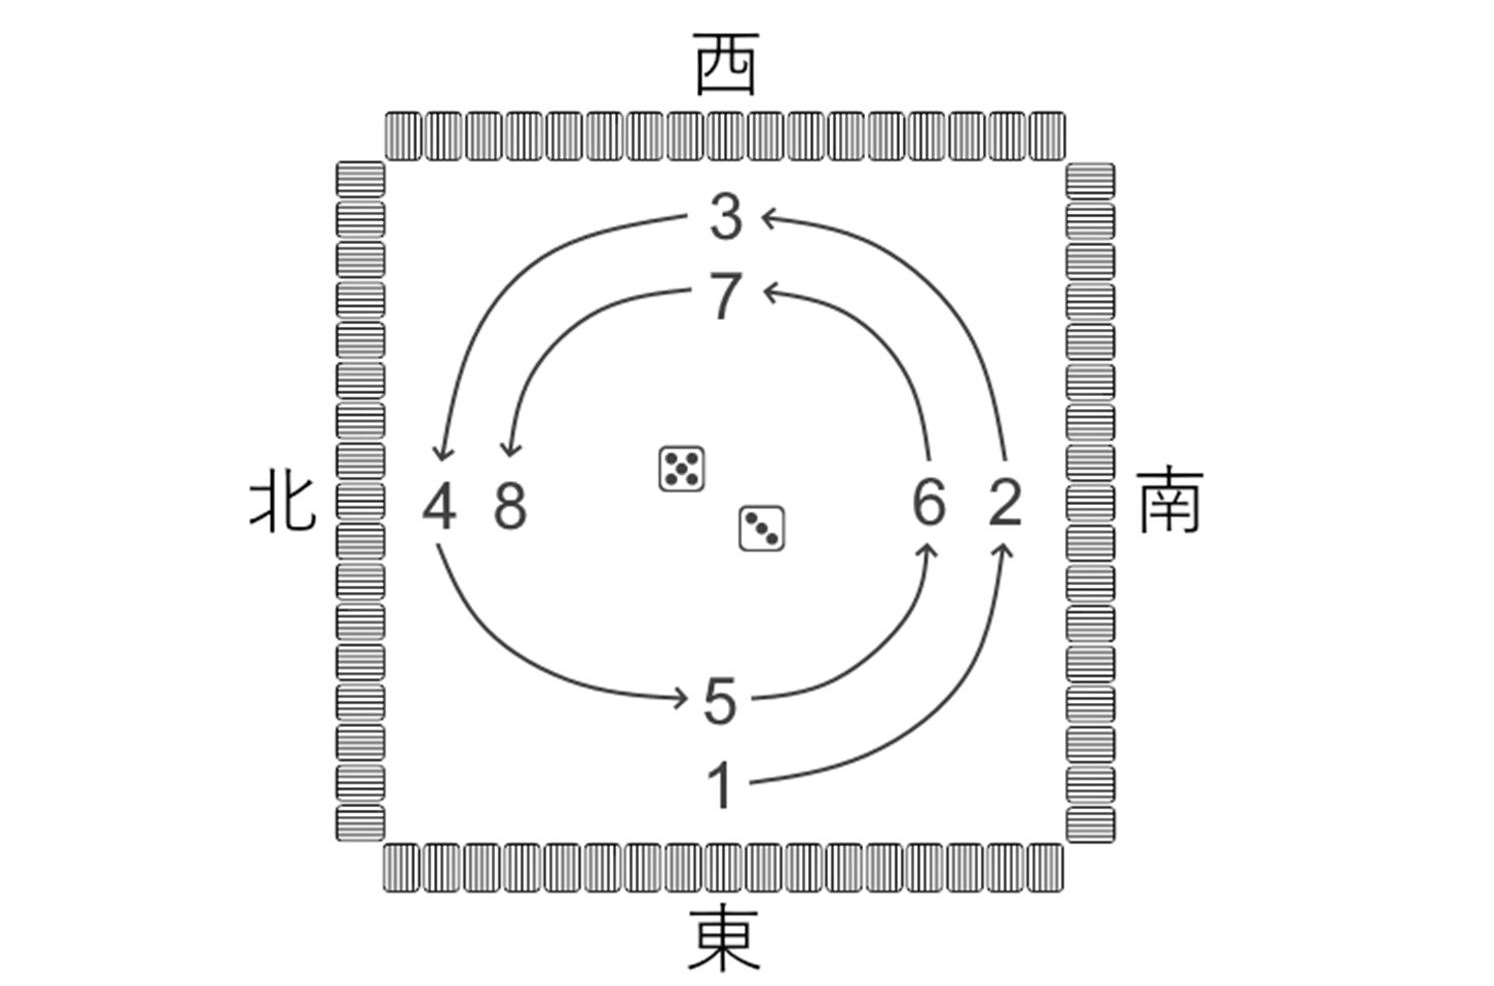
\includegraphics[width=16cm]{table-deal-start.png}
	\caption{Определение разлома стены}
\end{figure}

Затем игрок, на чью сторону указал дилер (в примере выше – север) отсчитывает от правого конца своей стороны стены столько тайлов, какое число выпало на кубиках до этого (в примере – 8) и немного отодвигает их от соседних тайлов вправо, создавая разлом стены. После этого он отсчитывает от разлома в обратную сторону 7 тайлов и делает второй разлом, обособляя получившуюся группу из 14 тайлов (см. рис.2). Эта группа называется мёртвой стеной и не разбирается в процессе игры. Оставшаяся часть стены называется живой стеной и используется во время раздачи для получения игроками тайлов (наподобие колоды карт). Разбирается она стопками верхний-нижний по часовой стрелке, начиная с верхнего тайла первой стопки после разлома и заканчивая нижним последней перед мёртвой стеной. Стена считается непрерывной, и переход через углы не имеет никакого значения как при формировании мёртвой стены, так и при последующем разборе.

Третий верхний тайл от конца мёртвой стены переворачивается рубашкой вниз (на рисунке это 6 ман) и служит в данной раздаче индикатором доры – тайла, дающего дополнительные очки при его наличии в руке. Подробно о дорах и принципе работы индикаторов рассказано в разделе VIII.

\begin{figure}[H]
	\centering
	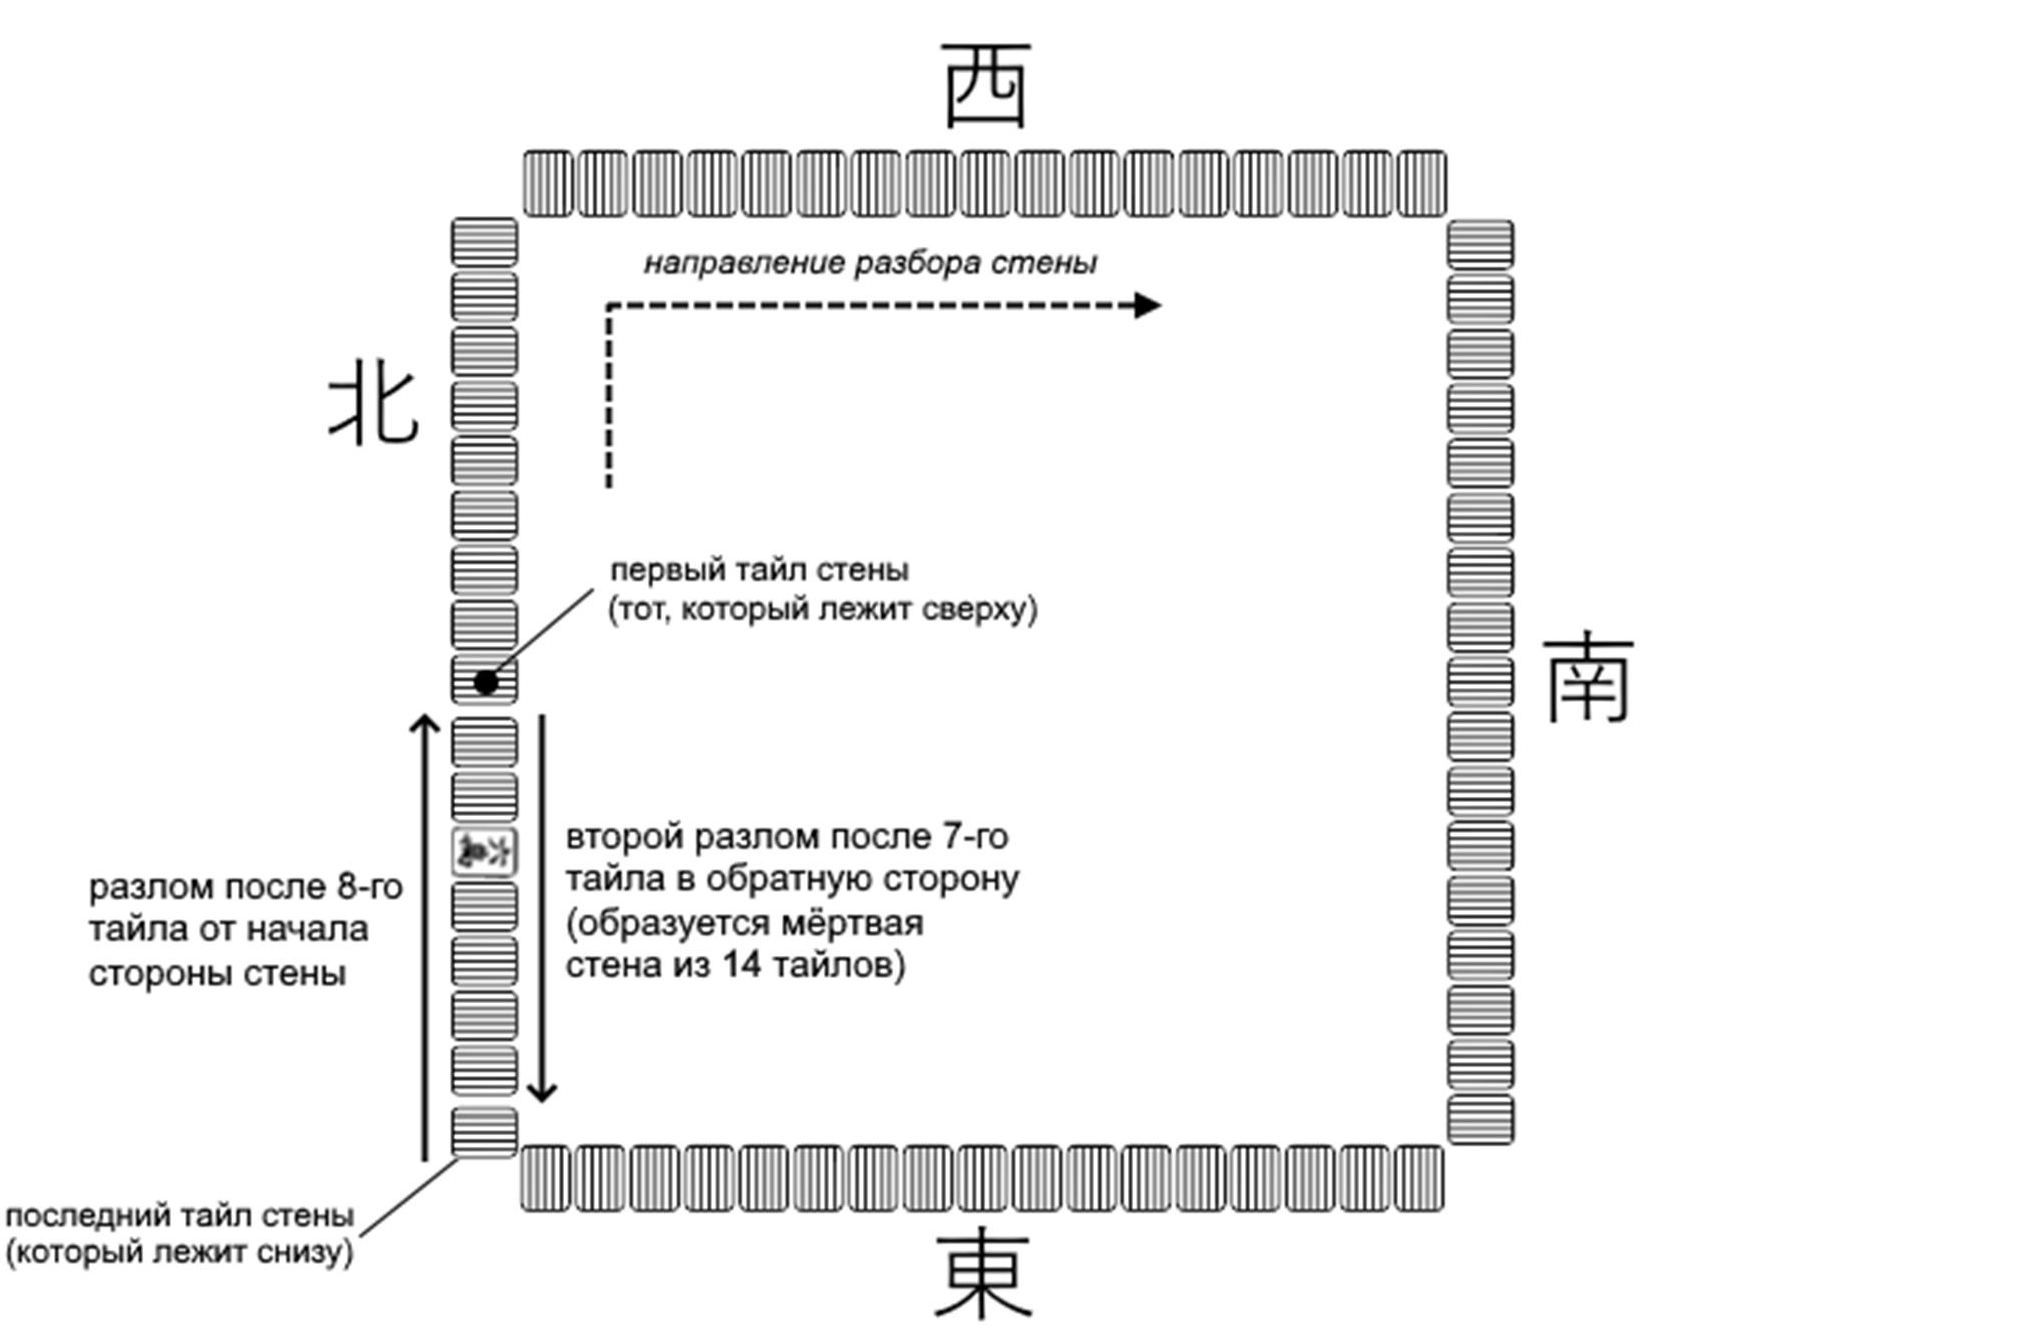
\includegraphics[width=16cm]{table-deal-start-2.png}
	\caption{Мертвая и живая стены}
\end{figure}

После открытия индикатора доры игроки берут себе со стены тайлы в стартовые руки. Начиная с дилера по очереди против часовой стрелки игроки начинают брать от начала живой стены по четыре тайла (две стопки по 2), пока у каждого не окажется 12 тайлов. После этого игроки в том же порядке берут ещё по одному тайлу (порядок разбора – всегда от верхнего к нижнему), а затем дилер берёт себе ещё один тайл (см. рис.3). Таким образом, в начале раздачи дилер имеет 14 тайлов, а остальные – по 13. Тайлы своих рук игроки расставляют перед собой в ряд вертикально изображением к себе, так, чтобы остальные видели только их рубашки. Для удобства игроки сортируют руки: ставят рядом тайлы одной масти по порядку номеров и одинаковые благородные тайлы. Допустим, игрок взял себе в стартовую руку следующие тайлы:

\mahjong{5m 6s 4m 8s 3z 9m 7z 2z 1s 3m 7z 7s 4m}

Он может отсортировать их следующим образом:

\mahjong{1s 678s 34459m 2377z}

Разные масти могут быть отсортированы слева направо или справа налево, а разные благородные тайлы могут стоять в разных местах – всё зависит от удобства для игрока и времени, затрачиваемого на сортировку.

В компьютерном маджонге построение стены, её разлом, набор и сортировка стартовых рук как правило происходят автоматически, и когда начинается раздача игроки сразу же видят свои отсортированные стартовые руки и индикатор доры. 

\begin{figure}[H]
	\centering
	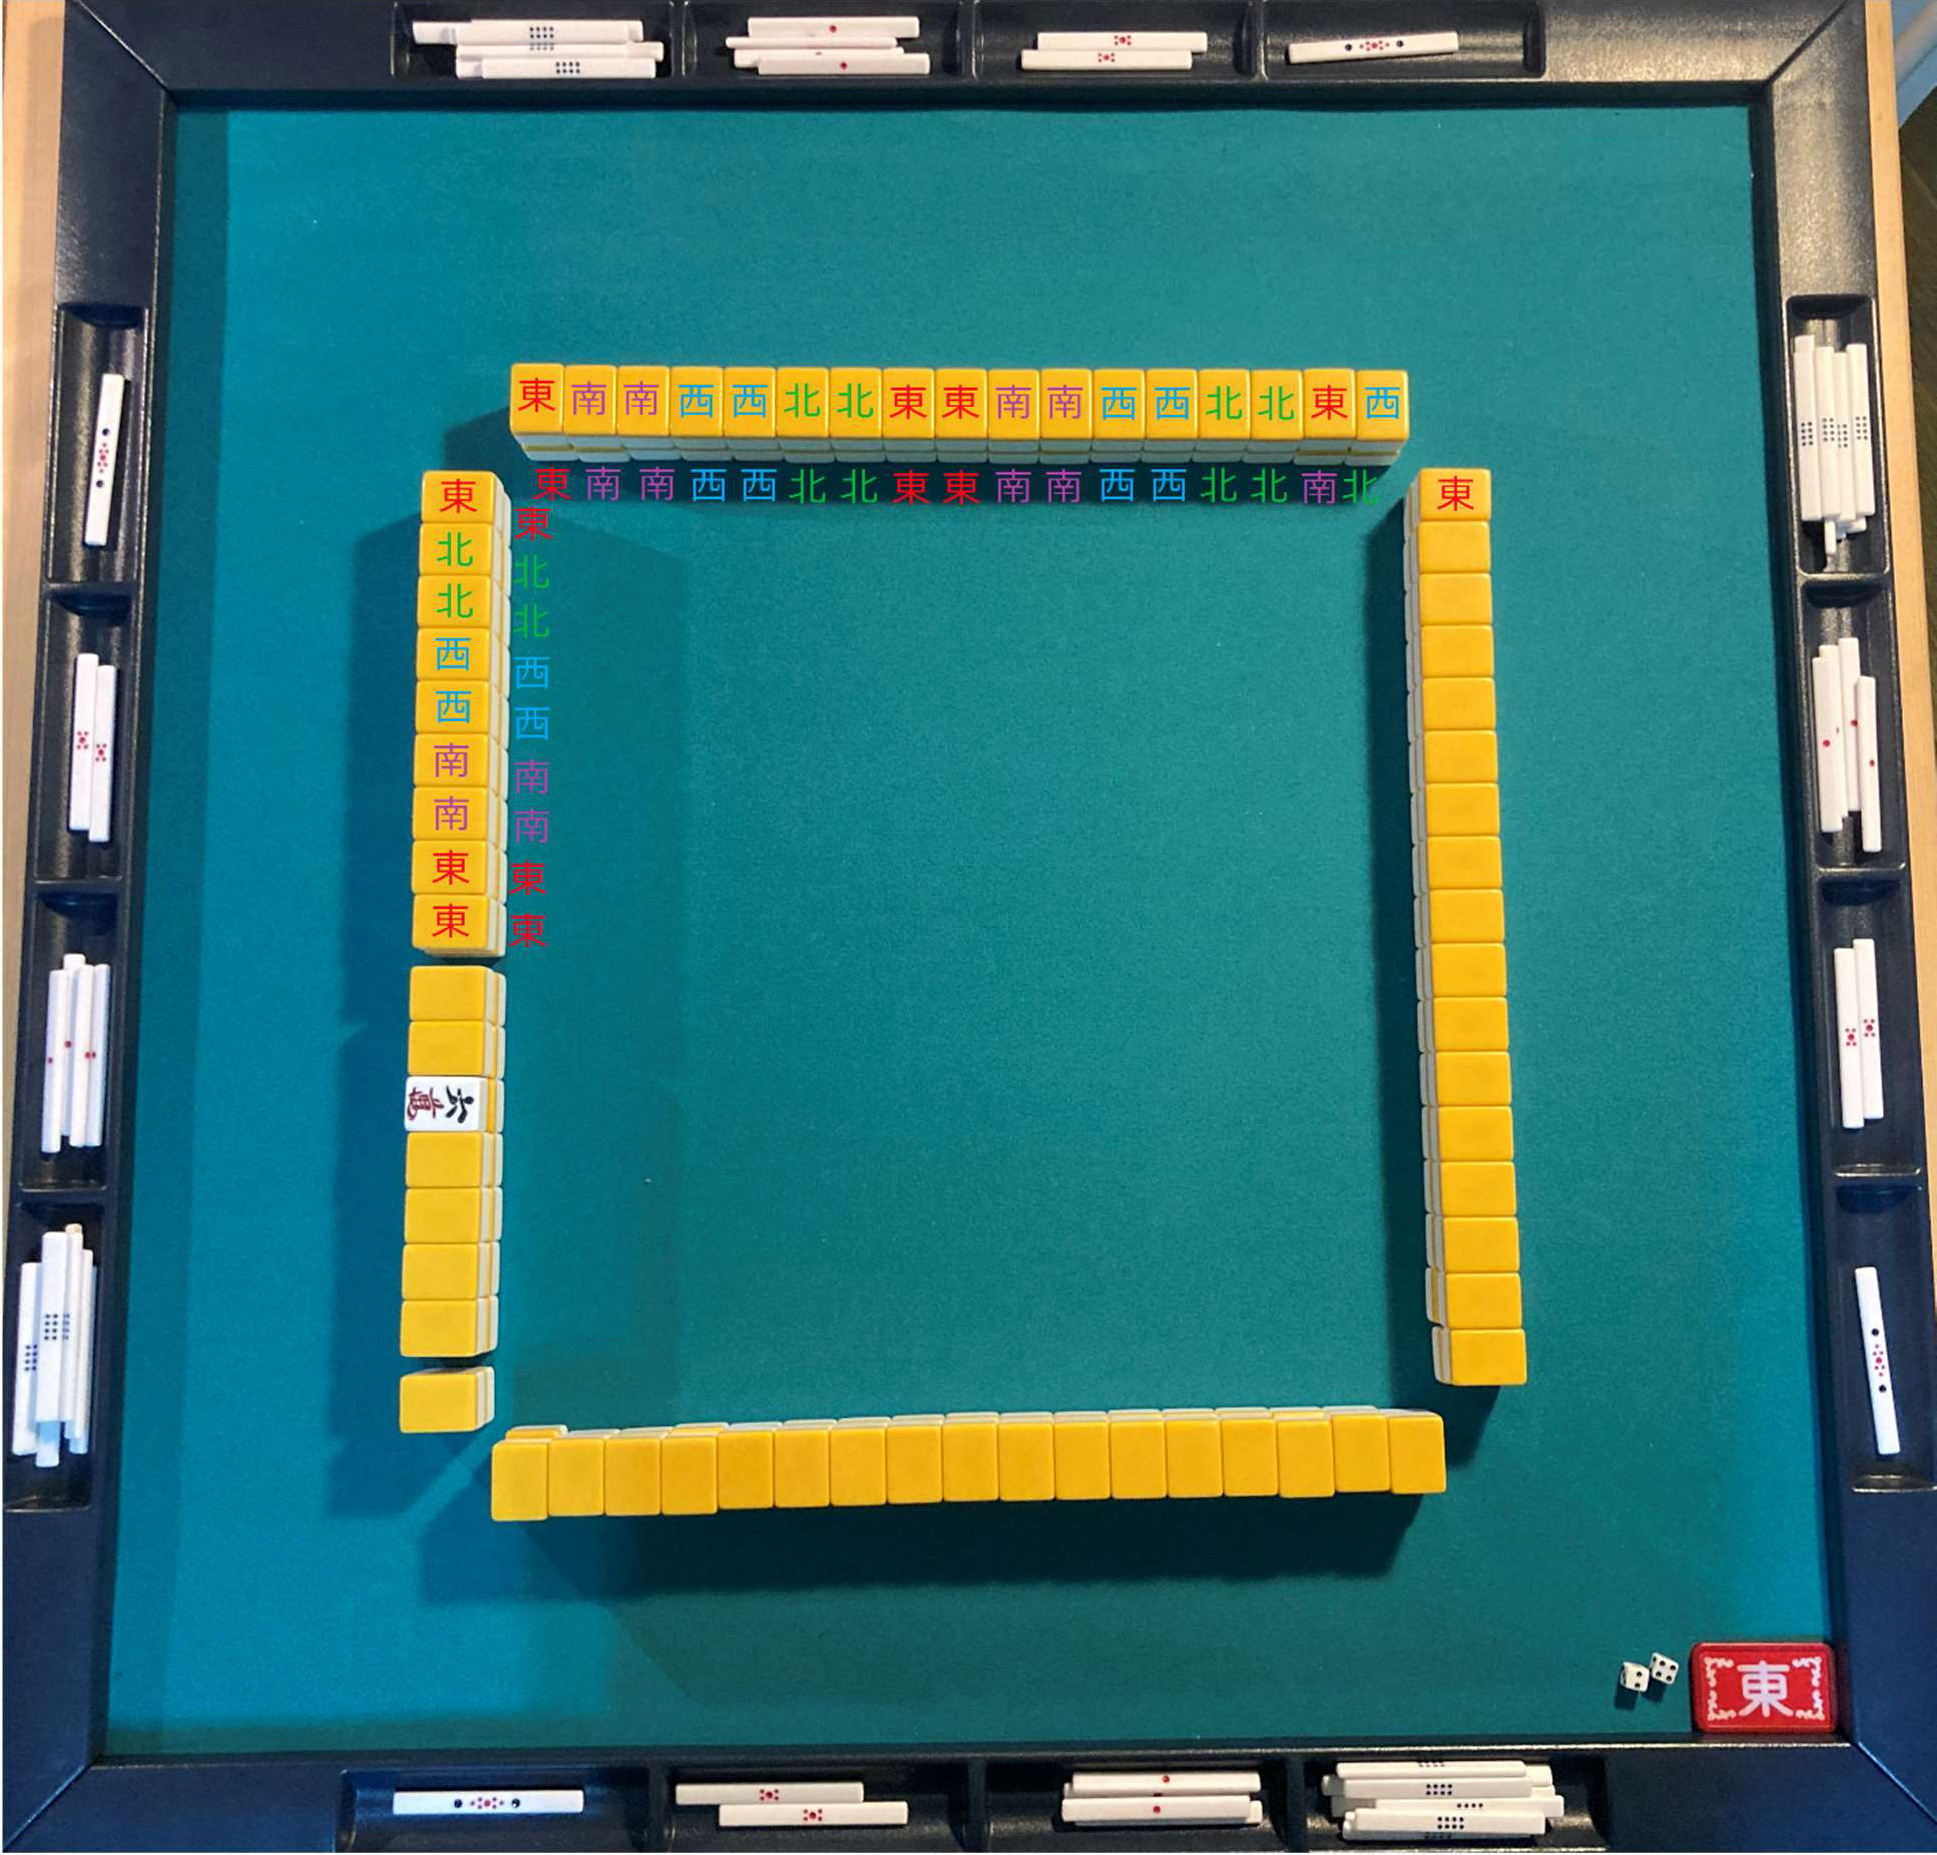
\includegraphics[width=16cm]{table-deal-start-3.png}
	\caption{Порядок разбора стены, фото}
\end{figure}

Обратите внимание на подписи тайлов - они показывают, какой игрок должен их взять (верхние тайлы стены подписаны прямо на рубашке, нижние – рядом). Предположим, что сейчас идёт первая раздача восточного раунда: индикатор первого дилера повёрнут иероглифом востока кверху, а кубики как индикатор текущего дилера лежат рядом с ним, т. е. первый дилер является дилером в этой раздаче.

\subsection{Ход раздачи}

В ходе раздачи, которая начинается сразу же после набора и сортировки всеми стартовых рук, игроки изменяют состав своих рук, набирая в них по одному новые тайлы с живой стены и выбрасывая ненужные. Цель каждого игрока в раздаче – собрать в руке четыре сета и одну пару (два одинаковых тайла). При объявлении кем-либо победы с готовой рукой раздача заканчивается. Цель всей игры – набрать как можно больше очков, получаемых в основном за собранные руки.

Сет – это определённая комбинация из трёх или четырёх тайлов. Они бывают трёх видов:
\begin{itemize}
	\item Три одинаковых тайла - \textit{пон};
	\item Четыре одинаковых тайла – \textit{кан};
	\item Последовательность из трёх тайлов одной масти подряд (по типу 1-2-3, 3-4-5 и т. п.) – \textit{чи}. Последовательности можно собирать только из тайлов мастей, и в них не должно быть перехода через девятку: 8-9-1 и 9-1-2 не засчитываются как чи.
\end{itemize}

Один тайл не может одновременно входить в два сета. В примере ниже в руке уже есть готовый пон из 4 ман, чи 7-8-9 ман и пара красных драконов, но последовательность 3-4-5-6-7 пин не засчитывается за два чи: для завершения этой формы в два сета требуется получить ещё один тайл (2, 5 либо 8 пин).

\mahjong{444789m 34567p 77z}

В руке из примера выше 13 тайлов, как и в любой руке не-дилера в начале раздачи, но выигрышная рука должна содержать как минимум 14 тайлов (3+3+3+3+2, если же в руке есть каны, число тайлов может доходить до 18). Четырнадцатый тайл игроки получают в свои ходы во время раздачи: раздача начинается с хода дилера, который сбрасывает из руки один из своих 14 тайлов, кладя его рубашкой вниз в центр стола; затем ход переходит к следующему игроку против часовой стрелки, который берёт первый тайл из оставшейся части живой стены и также сбрасывает один тайл из своей руки (можно сбрасывать и тайл, только что взятый со стены – такой сброс называется \textit{цумогири}). Затем ход переходит к следующему игроку, и так раздача продолжается до тех пор, пока кто-либо не соберёт руку и объявит победу, или же пока в живой стене не закончатся тайлы. 

Ходы в риичи-маджонге обязательны, пропускать взятие со стены либо сброс нельзя. Каны, а вместе с ними и руки, содержащие более 14 тайлов, возможно образовать специальными объявлениями, о которых рассказывается в следующем разделе. Ходы четырёх игроков, начиная от дилера, образуют круг раздачи. После окончания круга ход вновь переходит к дилеру, и начинается следующий круг. Группы сброшенных тайлов в центре стола называются сбросами или \textit{дискардами}. Каждый игрок имеет свой отдельный дискард. Тайлы следует выкладывать в сброс слева направо тремя рядами по 6 штук (начиная с ближнего к центру стола и далее по направлению к себе); четвёртый же ряд чаще не начинают, а вместо этого продолжают третий.

\begin{figure}[H]
	\centering
	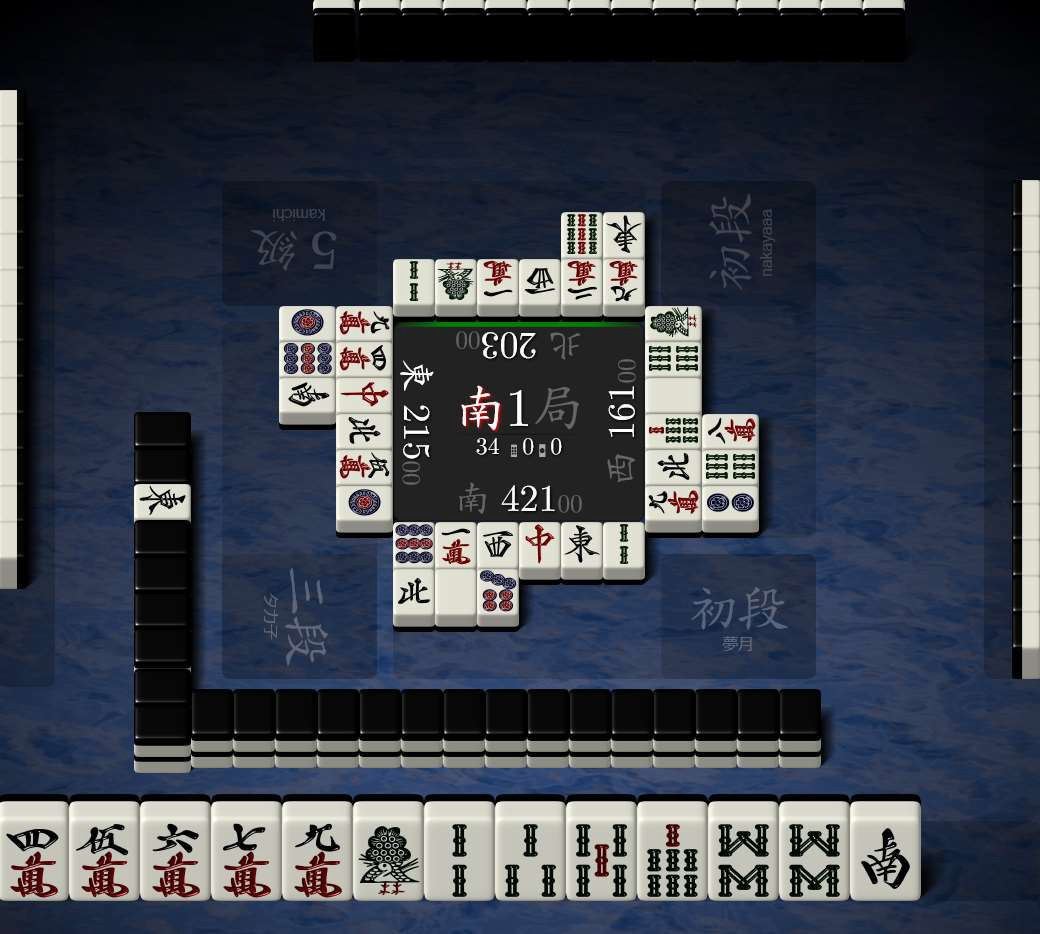
\includegraphics[width=16cm]{tenhou-deal.jpg}
	\caption{Пример раздачи на сервере tenhou.net}
\end{figure}

Рассмотрим вид стола в процессе раздачи на онлайн-сервере tenhou.net (рис.4). В центре – указатель раунда и номера раздачи за раунд (южный, первая) и указатели мест игроков со счётчиками очков (мы юг с 42100 очков; на онлайн-серверах вместо палочек используются цифровые счётчики). Вокруг центра – дискарды игроков, ниже – живая стена, слева – мёртвая стена с индикатором доры восточным ветром. По краям стола расположены руки игроков. Сейчас 9-й круг, ход севера: он получил тайл со стены, но ещё не совершил сброс. Пришедший со стены тайл сначала ставят отдельно (здесь он стоит слева от основной руки, если смотреть от нас), и встраивают в руку только после сброса, если сброшен другой тайл.

\subsection{Объявления в игре}

% TODO: Сорокин

Раздел в работе. Проверить, что следующие моменты описаны в разделе при его добавлении:

Риичи: единственное объявление, которое не прерывает круг. Важное уточнение для последующих объяснений.

Кан при риичи: не может менять интерпретацию руки (но может менять список яку, например, игрок может получить санканцу сверху).

Дабл-рон и трипл-рон: есть. 

Невыигравшие палки при даблроне: отдаются первому по ходу раздачи победившему. Выигравшие палки возвращаются объявившим.

Хонба при даблроне платится всем победителям в полном объеме.

При даблроне/триплроне невалидный рон наказывается вежливым указанием, при повторе может быть назначен штраф.

Куикаэ: не допускается ни в каком виде

\subsection{Фуритен и временный фуритен}

Правило \textit{фуритен} (\textnihon{フリテン}), или правило упущенного сброса, запрещает игроку объявлять рон, если хоть один из выигрышных тайлов, завершающих руку, лежит у него в дискарде. При этом как дискард учитываются и тайлы, взятые оттуда для сетов другими игроками. Именно из-за этого при объявлениях сетов требуется указывать какой тайл был взят и с кого из противников, кладя один из тайлов боком с соответствующей стороны.

Например, рассмотрим игрока со следующей рукой:

\mahjong{33456678m 23p 678s}

Предположим, дискард у игрока следующий:

\mahjong{1p 4z 7z 2s 4s 9m}

В данном случае игрок не может объявить рон ни при сбросе противником 1 пин, ни при сбросе 4 пин, потому что в его дискарде есть «упущенный» выигрышный тайл 1 пин. При этом ограничений на объявление цумо нет. Если игрок перестроит свою руку так, чтобы сброшенные в дискард тайлы не завершали выигрышное ожидание, фуритен перестанет действовать, и он снова сможет объявлять рон. Например, это будет возможно если руку выше изменить следующим образом взятием 5 пин и сбросом 2 пин: 

\mahjong{33456678m 35p 678s}

В этом случае ожидание на 1 пин пропадёт, и игрок сможет объявить рон на сброшенную кем-либо 4 пин. 

Фуритен даёт возможность для игры в защиту: тайлы, лежащие в сбросе у противника, можно уверенно сбрасывать, не опасаясь, что он объявит на них рон (при победе по рону игрок получает очки за счёт сбросившего выигрышный тайл; о выплатах см. раздел IX). Есть и более продвинутые приёмы защиты, основанные на фуритене, которым посвящены отдельные специализированные статьи, в данном руководстве не рассматриваемые.

\textit{Временный фуритен} – это отдельное правило, которое не позволяет игроку объявлять рон, если на текущем круге считая от хода игрока уже был сброшен какой-либо из выигрышных для него тайлов. Действие временного фуритена заканчивается с первым же ходом игрока – в момент, когда игрок формально может сменить ожидание. Допустим у нас на нашем ходу имеется следующая рука:

\mahjong{123456789m 99s 11z}

В случае если игрок справа сбросил 9 со и мы пропустили возможный рон, а сразу за ним игрок напротив сбрасывает восток или ещё одну 9 со, объявлять рон на этот тайл нельзя, потому что на этом круге рон уже был пропущен. Если же кто-то ещё раз сбросит 9 со или восток уже после следующего нашего хода, рон объявить будет можно.

Временный фуритен существует для предотвращения избирательности в объявлении рона, но иногда действует во вред игрокам в темпае, если после одного пропущенного выигрышного тайла на том же круге сбрасывается тайл, дающий руке большую стоимость, чем первый. Если игрок пропустил один рон после объявления риичи, из-за временного фуритена он не может победить по рону до конца раздачи, т. к. после риичи сменить ожидание невозможно (подробно о риичи рассказывается в посвящённом ему разделе VII).

\subsection{Яку: условия победы}

Для объявления победы необходимы не только четыре сета и пара в руке, но и выполнение хотя бы одного \textit{яку} – условия победы, приносящего руке стоимость. Рука без яку не имеет стоимости, и \lineunder{с такой рукой объявлять победу нельзя}, даже если собраны все сеты и пара. Яку бывают двух типов: это либо наличие определённых комбинаций тайлов в руке, либо особые игровые ситуации, при которых происходит победа. Стоимость яку измерима: каждое из них имеет фиксированную стоимость в \textit{ханах} (яп. \textnihon{飜} или \textnihon{翻}) – специальных единицах, используемых для удобства, которые при подсчёте общей стоимости руки переводятся в очки.

Яку бывают \textbf{комбинационными} и \textbf{ситуационными}. 

Комбинационные яку даются за сочетания тайлов в руке, объединенные некоторым общим принципом. Яку может давать как часть руки (например, в случае комбинации \textit{якухай} яку дается за любой пон драконов или ветров места или раунда), так и вся рука полностью - в случае выполнения некоторого условия для всей руки без исключения (например, яку \textit{тойтой} дается в случае если вся рука состоит только из понов). 

Ситуационные яку даются за выполнение некоторых игровых условий, не связанных с формой руки (например, \textit{риншан кайхо} дается за победу с замещающего тайла при объявлении кана).

Полный список яку с подробным описанием приведен в приложении.

Яку можно сочетать друг с другом – в таких случаях стоимости всех яку в руке суммируются (за некоторыми исключениями; все исключения описаны в приложении).

Некоторые яку невозможно сочетать, потому что их условия противоречат друг другу. Например, \textit{чанта} не сочетается с \textit{тан'яо}, потому что требует наличия крайних или благородных тайлов, которых в руке с тан'яо быть не может. В других случаях теоретически возможные сочетания яку запрещены правилами.

Некоторые яку требуют специфических ожиданий - в этом случае при победе игрокам запрещается встраивать выигрышный тайл в руку – иначе другие игроки после открытия руки не смогут его проверить.

\subsubsection{Якуманы}

Некоторые яку, называемые \textit{якуманами}, собираются настолько редко и тяжело, что стоят максимально возможное количество очков (32000 очков для не-дилера и в 48000 для дилера). Якуманы не сочетаются ни с какими яку, кроме других якуманов – именно поэтому их стоимость обычно считают сразу в очках, хотя можно записать её и в ханах – 13. Когда в руке несколько якуманов, они складываются, образуя двойные, тройные якуманы и т. д., а стоимость руки с каждым дополнительным якуманом возрастает ещё на 32000 / 48000 очков. Якуманы также бывают как комбинационными, так и ситуационными - полный список с описаниями можно найти в приложении.

\subsection{Дора}

Дора (\textnihon{ドラ}) – это тайл, наличие которого в руке увеличивает её стоимость на 1 хан. Однако дора не даёт яку, и с рукой без яку нельзя объявить победу даже если в ней есть доры. Дора в каждой раздаче определяется индикатором, который открывается в мёртвой стене перед её началом. Дорой считается следующий тайл после индикатора по порядку, указанному в разделе о наборе тайлов:
\begin{itemize}
	\item Тайлы мастей: 1→2→3→4→5→6→7→8→9→1 (дора только в той же масти, что и индикатор);
	\item Ветра: \textnihon{東}→\textnihon{南}→\textnihon{西}→\textnihon{北}→\textnihon{東};
	\item Драконы: красный→белый→зелёный→красный.
\end{itemize}

Например, если индикатор – 2 пин, дорой является 3 пин; если индикатор 9 соу, дора – 1 соу; если красный дракон, то дорой будет белый.
Когда в руке есть несколько экземпляров дор, их стоимость складывается:

\mahjong{233445m 567p 4599s-3s}

Мертвая стена:
\mahjong{XX3mXXXX}

Эта рука без ситуационных яку будет стоить 3 хан: один за пинфу и ещё по одному за две доры 4 ман.

Помимо «обычных» дор существуют дополнительные, многие из которых ранее уже упоминались. За каждый экземпляр любой из них даётся дополнительный хан, как и за обычную дору:
\begin{itemize}
	\item \textit{Кандоры}. При объявлении любого кана в мёртвой стене открывается один индикатор кандоры (соседний тайл с индикатором доры с той стороны, где от него до конца стены 4 тайла). Всего их может быть открыто 4, по числу тайлов от индикатора доры до конца мёртвой стены (пятый кан за раздачу объявлять запрещено). Сколько в раздаче объявлено канов, столько и открыто индикаторов кандор. Индикаторы работают точно так же, как и обычные.
	\item \textit{Урадоры}. При победе после объявления риичи, тайл, находящийся в мёртвой стене под индикатором доры, открывается и становится дополнительным индикатором доры, которая называется урадорой. Если в выигранной руке риичи-игрока оказываются урадоры, он получает за них дополнительную стоимость. Индикаторы открывает лично выигравший руку с риичи игрок либо игрок, со стороны которого находится мёртвая стена.
	\item \textit{Кан-урадоры}. Если во время раздачи объявлялись каны, при победе после риичи открывается и становится индикатором не только тайл под индикатором доры, но и все тайлы под открытыми индикаторами кандор. Например, если за раздачу было объявлено два кана, урадор будет три: одна обычная и две кан-урадоры.
\end{itemize}

Таким образом, все тайлы мёртвой стены, кроме добавляемых в неё из живой стены после объявления канов, теоретически могут быть использованы в игре либо как тайлы замены, либо как индикаторы дор (см. схему мёртвой стены в разделе IV).

Также в данных правилах регламентируются \textit{акадоры}: рисунок на некоторых экземплярах пятёрок мастей сделан полностью красным, и каждая такая пятёрка в руке увеличивает её стоимость на 1 хан. Акадор в наборах три, по одной в каждой масти. Использование акадор в наборах является обязательным, если иное не указано в сопутствующем регламенте конкретного турнира из-за обстоятельств непреодолимой силы (например, в случае, если у организаторов недостаточно наборов с акадорами).

Если несколько одинаковых индикаторов доры указывают на один и тот же тайл, он становится двойной, тройной или четверной дорой по числу указывающих индикаторов, и такие доры дают соответственно 2, 3 или 4 дополнительных хана за каждый тайл. Если индикатор указывает на пятёрку, стоимость акадоры также увеличивается на 1 хан:

\mahjong{788m24056p246s22z}

Мертвая стена:
\mahjong{XX1z4p1zXX}

Эта рука содержит дор на 7 хан.

\subsection{Подсчёт стоимости руки и порядок выплат}

Стоимость руки сначала считается как сумма всех ханов, полученных за яку и доры, и всех фу (\textnihon{符}) – «мини-очков», начисляемых за определённые сеты в руке, форму ожидания на выигрышный тайл и другие мелкие особенности руки, не дающие яку. После этого стоимость, выраженная в ханах и фу (например, 2 хан 40 фу), переводится в очки по специальной таблице или формуле, которые будут рассмотрены далее.

Мини-очки \textit{фу} поощряют игрока за мелкие сложности в сборе руки, не дающие новых яку. Они считаются после подсчёта суммарного количества ханов за яку и доры. Если в руке 5 хан или больше, фу считать не нужно: стоимость такой руки в очках будет зависеть только от количества ханов.
Фу начисляются за поны и каны в руке, якухайные пары, ожидание на выигрышный тайл и тип победы. Каждая рука, если она стоит менее 5 хан, по умолчанию имеет 20 фу, и все остальные полученные фу складываются с ними. После подсчёта всех фу получившееся число округляется вверх до десятков (например, если при суммировании получилось 54 фу, итоговым значением будет 60). Единственное исключение – читойцу: любая рука из семи пар (опять же, если её общая стоимость – менее 5 хан) оценивается в 25 фу, никакие дополнительные фу к ним не прибавляются, и это число не округляется вверх до 30.

\subsubsection{Фу за поны и каны}

Количество фу зависит от открытости сетов (не всей руки!) и тайлов, из которых они состоят:

\begin{tabular}{|L{7cm}|C{3cm}|C{3cm}|}
	\hline
	& Открытый сет &
	Закрытый сет \\
	\hline
	Пон средних тайлов &
	+ 2 фу &
	+ 4 фу \\
	\hline
	Пон крайних или благородных тайлов &
	+ 4 фу &
	+ 8 фу \\
	\hline
	Кан средних тайлов &
	+ 8 фу &
	+ 16 фу \\
	\hline
	Кан крайних или благородных тайлов &
	+ 16 фу &
	+ 32 фу \\
	\hline
\end{tabular}

Фу начисляются за каждый отдельный пон и кан в руке в зависимости от его типа по таблице. Если пон образовался в руке с получением выигрышного тайла, он считается открытым, если тайл получен по рону, и закрытым, если по цумо. За чи, как более простые в сборе сеты, фу не даётся.

\subsubsection{Фу за якухайные пары}

Если в руке пара состоит из тайлов, сет которых дал бы якухай (драконы или ветра раунда/места), за такую пару начисляется 2 дополнительных фу. За пару совпадающих ветров раунда и места, сет которых дал бы двойной якухай, обычно даётся 4 фу. Всё это не относится к читойцу: такие руки всегда стоят 25 фу.

\subsubsection{Фу за тип победы}

\begin{itemize}
	\item При победе по рону с закрытой рукой даётся 10 дополнительных фу;
	\item При победе по цумо с любой рукой (открытой или закрытой) даётся 2 дополнительных фу, если эта рука не содержит пинфу\footnote{Можно заметить, что все условия для пинфу подобраны так, чтобы рука в итоге не получила фу кроме базовых 20: в ней нет ни коцу и канов, ни якухайных пар, ни ценных ожиданий. Действительно, буквальный перевод названия "пинфу" – это «рука без фу». Единственное исключение – +10 фу за рон на закрытой руке.}. При победе с тайла замены (риншан кайхо) 2 фу за цумо тоже не начисляются;
	\item При победе по рону с открытой рукой, в которой выполняются все остальные условия для пинфу (нет понов, канов и якухайных пар, ожидание в две стороны в рянмен) даётся 2 дополнительных фу. Других фу, кроме базовых, в такой руке нет, и поэтому она всегда стоит 30 фу.
\end{itemize}

\subsubsection{Фу за ожидание на выигрышный тайл}

В темпае возможны пять различных базовых форм ожидания выигрышного тайла, и некоторые, наиболее «неудобные» из них, оцениваются в дополнительные 2 фу:

\noindent\begin{tabular}{|C{3cm}|C{5cm}|C{3cm}|C{3cm}|}
\hline
	Название  &
	Пример формы &
	Выигрышные тайлы &
	Фу \\
\hline
	\rule[0ex]{0pt}{5ex} Рянмен \newline (в две стороны) \newline &
	\mahjong{34p} &
	\mahjong{25p} &
	не начисляется \\
\hline
	\rule[0ex]{0pt}{5ex} Канчан \newline (в «дырку») \newline &
	\mahjong{35s} &
	\mahjong{4s} &
	+2 фу \\
\hline
	\rule[0ex]{0pt}{5ex} Пенчан \newline (краевое) \newline &
	\mahjong{12m} &
	\mahjong{3m} &
	+2 фу \\
\hline
	\rule[0ex]{0pt}{5ex} Танки \newline (в пару) \newline &
	\mahjong{3s} &
	\mahjong{3s} &
	+2 фу \\
\hline
	\rule[0ex]{0pt}{5ex} Сянпон \newline (в две пары) \newline &
	\mahjong{33z-11m} &
	\mahjong{3z1m} &
	не начисляется \\
\hline
\end{tabular}

За сянпон как ожидание фу не даётся, но 2, 4 или 8 фу начисляется за получившийся пон в соответствии с таблицей фу за сеты. Если выигрышный тайл пришёл одновременно в несколько ожиданий разного типа, считается только то, с которым рука получается дороже всего в очках (о пересчёте ханов и фу в очки см. следующий раздел) – это же касается и интерпретации сетов в руке. Например, если считать в руке ниже выигрышным ожиданием рянмен 5-6, а не пенчан 8-9, она получит дополнительный хан за  пинфу,  и поэтому будет выбрана такая интерпретация ожиданий. Соответственно, 2 фу за пенчан начислены не будут.

\mahjong{23466m 56789p 123s-7p}

В случае более сложных ожиданий, эти ожидания всегда можно свести к базовым и рассчитать соответствующую стоимость. Например, формы \textit{нобетан} и \textit{санментан} всегда ждут только в пару (пусть и несколько разновидностей тайлов), тогда как форма \textit{рянтан} может рассматриваться как рянмен и как танки (отсюда и название формы). Рассмотрим примеры таких форм.

\textbf{Нобетан}

\mahjong{3456p}

Эту форму можно рассмотреть как чи + ожидание в пару двумя способами:

\mahjong{3p-456p}

\mahjong{345p-6p}

\textbf{Санментан}

\mahjong{3456789s}

Тут аналогично, но способов уже три:

\mahjong {3s-456s-789s}

\mahjong{345s-6s-789s}

\mahjong{345s-678s-9s}

\textbf{Рянтан}

\mahjong{3444m}

Эту форму можно рассмотреть либо как пон + ожидание в пару, либо как пару + ожидание в две стороны:

\mahjong{3m-444m} 

\mahjong{34m-44m}

Существуют и другие комплексные формы ожиданий, но каждую из них можно разложить до базовых форм тем или иным способом.

\subsubsection{Примеры подсчёта ханов и фу в руке}

Пример №1.

\mahjong{123m99p13s-2s}\hfill \mahjong{8'79s 66'6z}

Мертвая стена:
\mahjong{XX9mXXXX}

(раунд южный, игрок на востоке, победа без ситуационных яку)

\begin{tabular}{lr}
	Якухай & 1 хан \\
	Открытая чанта & 1 хан \\
	Доры & 1 хан \\
	Базовые фу & 20 фу \\
	Открытый пон благородных тайлов & 4 фу \\
	Ожидание в канчан & 2 фу \\
	\hline
	\textbf{Итого} & \textbf{3 хан 30 фу} \\
\end{tabular}

Пример №2.

\mahjong{340567m 44s 22z-4s} \hfill \mahjong{X99mX}

Мертвая стена: \mahjong{XX2p3zXXX}

Нижний ряд мертвой стены: \mahjong{XX6m9pXXX}

(раунд восточный, игрок на юге, победа по риичи без иппацу и других ситуационных яку с другого игрока)

\begin{tabular}{lr}
	Риичи & 1 хан \\
	Акадора & 1 хан \\
	Урадора & 1 хан \\
	Базовые фу & 20 фу \\
	Закрытый кан крайних тайлов & 32 фу \\
	Открытый пон средних тайлов (4 соу) & 2 фу \\
	Якухайная пара & 2 фу \\
	Закрытый рон & 10 фу \\
	\hline
	\textbf{Итого} & \textbf{3 хан 70 фу} \\
\end{tabular}

Пример №3. 

\mahjong{455667p3z-3z}

Мертвая стена: \mahjong{XX3p4s3pXX}

(раунд южный, игрок на севере, победа с тайла замены)

\begin{tabular}{lr}
	Якухай & 1 хан \\
	Открытое хон'ицу & 2 хан \\
	Риншан кайхо & 1 хан \\
	Доры & 2 хан \\
	\multicolumn{2}{l}{В руке больше 4 хан, фу не подсчитываются} \\
	\hline
	\textbf{Итого} & \textbf{6 хан} \\
\end{tabular}

Пример №4.

\mahjong{5688m 456p 678s-4m} \hfill \mahjong{4'23p}

Мертвая стена: \mahjong{XX6mXXXX}

(раунд восточный, игрок на востоке, победа без ситуационных яку)

\begin{tabular}{lr}
	Тан'яо & 1 хан \\
	Базовые фу & 20 фу \\
	Рон с «открытым пинфу» & 2 фу \\
	\hline
	\textbf{Итого} & \textbf{1 хан 30 фу} \\
\end{tabular}

Пример №5.

\mahjong{222m 678p 1406888s-1s}

Мертвая стена: \mahjong{XX4zXXXX}

(раунд южный, игрок на западе, победа с закрытым цумо без других ситуационных яку)

\begin{tabular}{lr}
	Мензен цумо & 1 хан \\
	Акадора & 1 хан \\
	Базовые фу & 20 фу \\
	Два закрытых пона средних тайлов & 8 фу \\
	Ожидание в танки (в пару) & 2 фу \\
	Цумо & 2 фу \\
	\hline
	\textbf{Итого} & \textbf{2 хан 40 фу} \\
\end{tabular}

\subsubsection{Подсчет очков в руке}

В риичи-маджонге все игроки начинают игру с 30000 очков, и в процессе игры только обмениваются очками друг с другом: больше очки ниоткуда не появляются и никуда не исчезают. Поэтому сумма очков за столом всегда равна 120000.

Выплаты за собранные руки производятся сразу после объявления победы и подсчёта очков, перед началом следующей раздачи. После рона всю стоимость руки победителю выплачивает игрок, сбросивший выигрышный тайл, а при цумо выплата делится между всеми тремя оставшимися игроками. При двойном или тройном роне набросивший игрок платит всем победителям.

Победитель раздачи должен после показа руки противникам назвать стоимость руки в очках; опционально также перед этим перечислить яку и назвать число дор, например, «иццу, хон’ицу, одна дора – 7700». Если в руке возможны несколько интерпретаций сетов с разными стоимостями, выбрать нужно самую дорогую по стоимости в очках (о переводе ханов и фу в очки см. далее). Пример (победа не-дилера без риичи и других ситуационных яку, кроме мензен цумо, дор также нет):

\mahjong{777888999p23m99m-4m}

Если считать форму в пинах за три чи 7-8-9, то это пинфу, ипейко, мензен цумо – 3 хана 20 фу, 2700 очков. Если же за три пона, то это сан’анко и мензен цумо – 3 хана 40 фу, 5200 очков. Рука должна быть посчитана по варианту с сан’анко.

Для перевода ханов и фу в очки пользуются таблицей выплат. Далее приведена небольшая часть этой таблицы для самых частых стоимостей рук, а полную таблицу можно найти в приложении в конце правил. Для рук дилера используется отдельная таблица: рука дилера всегда стоит примерно в полтора раза больше очков, чем рука не-дилера с таким же количеством ханов и фу. Однако при цумо другого игрока дилер выплачивает примерно в два раза большую долю стоимости руки, чем не-дилер. При цумо дилера все выплачивают равные части стоимости.

В каждой ячейке сверху большими цифрами указана выплата при победе по рону, ниже – выплаты каждого из игроков при цумо: в не-дилерской таблице после дроби указана выплата дилера, перед дробью – каждого из оставшихся игроков, а в дилерской есть только одно число – выплата каждого из трёх остальных игроков. Например, если дилер возьмёт цумо с рукой в 2 хан 40 фу, каждый заплатит ему по 1300 очков, и вся рука будет стоить 3900. При цумо не-дилера с рукой в 1 хан 30 фу дилер заплатит ему 500 очков, а оставшиеся два игрока – по 300, и вся рука будет стоить 1100 очков.

Если в ячейках стоят прочерки, это значит, что такого количества ханов и фу при соответствующем типе победы в руке не может быть. В этом можно убедиться, вспомнив, с какими яку рука может иметь такое количество фу: 20 фу – это пинфу-цумо без дополнительных фу за рон (минимум 2 хан из-за мензен цумо), а 25 фу – это читойцу, которое тоже невозможно получить по цумо без дополнительного хана за мензен цумо.

\noindent\begin{tabular}{ |C{1.5cm}|C{2cm}|C{2cm}|C{2cm}|C{2cm}|C{2cm}|C{2cm}| }
	\hline
	Не-дилер &
	20 фу &
	25 фу &
	30 фу &
	40 фу &
	50 фу &
	60 фу \\
\hline
	1 хан &
	– \linebreak
	– &
	– \linebreak
	– &
	1000 \linebreak
	300 / 500 &
	1300 \linebreak
	400 / 700 &
	1600 \linebreak
	400 / 800 &
	2000 \linebreak
	500 / 1000 \\
\hline
	2 хан &
	– \linebreak
	400 / 700 &
	1600 \linebreak
	– &
	2000 \linebreak
	500 / 1000 &
	2600 \linebreak
	700 / 1300 &
	3200 \linebreak
	800 / 1600 &
	3900 \linebreak
	1000 / 2000 \\
\hline
	3 хан &
	– \linebreak
	700 / 1300 &
	3200 \linebreak
	800 / 1600 &
	3900 \linebreak
	1000 / 2000 &
	5200 \linebreak
	1300 / 2600 &
	6400 \linebreak
	1600 / 3200 &
	7700 \linebreak
	2000 / 3900/ \\
\hline
	4 хан &
	– \linebreak
	1300 / 2600 &
	6400 \linebreak
	1600 / 3200 &
	7700 \linebreak
	2000 / 3900 &
	8000 \linebreak
	2000 / 4000 & & \\

	\hline
\end{tabular}

\noindent\begin{tabular}{ |C{1.5cm}|C{2cm}|C{2cm}|C{2cm}|C{2cm}|C{2cm}|C{2cm}| }
	\hline
	Дилер &
	20 фу &
	25 фу &
	30 фу &
	40 фу &
	50 фу &
	60 фу \\
\hline
	1 хан &
	– \linebreak
	– &
	– \linebreak
	– &
	1500 \linebreak
	500 &
	2000 \linebreak
	700 &
	2400 \linebreak
	800 &
	2900 \linebreak
	1000 \\
\hline
	2 хан &
	– \linebreak
	700 &
	2400 \linebreak
	– &
	2900 \linebreak
	1000 &
	3900 \linebreak
	1300 &
	4800 \linebreak
	1600 &
	5800 \linebreak
	2000 \\
\hline
	3 хан &
	– \linebreak
	1300 &
	4800 \linebreak
	1600 &
	5800 \linebreak
	2000 &
	7700 \linebreak
	2600 &
	9600 \linebreak
	3200 &
	11600 \linebreak
	3900 \\
\hline
	4 хан &
	– \linebreak
	2600 &
	9600 \linebreak
	3200 &
	11600 \linebreak
	3900 &
	12000 \linebreak
	4000 & & \\

\hline
\end{tabular}

В таблицах можно заметить закономерность: \textbf{удвоение фу эквивалентно +1 хану}. Эту закономерность полезно знать для лучшего запоминания, кроме того она позволяет быстро рассчитать очки для рук с большим числом фу, например рука стоимостью в 1 хан и 100 фу будет иметь точно ту же стоимость, что и рука в 2 хан 50 фу, и ту же стоимость, что и рука в 3 хан 25 фу. Почему так происходит? 

Значения выплат в таблице получены по \textbf{одной и той же формуле}. Во время игры можно пользоваться таблицей, и поэтому знать формулу не нужно, но она может быть полезна для понимания принципов перевода ханов и фу в очки. Выглядит она так:

\begin{equation}
	\large
	Base = Fu \cdot 2 ^ {Han + Bazoro}
\end{equation}

\textit{Бадзоро} - это базовый коэффициент, обычно равный двум. В данных правилах бадзоро всегда имеет именно такое значение.

Из базового значения легко получить конкретное количество очков по простой формуле:

\begin{equation}
	\large
	Points = \lceil Base * k \rceil
\end{equation}

Обратите внимание на округление вверх до сотен - оно производится \textit{после} умножения базы на коэффициент \textit{k}. 

\textit{k} – это коэффициент, зависящий от типа победы и дилерства победителя:
\begin{itemize}
	\item При не-дилерском роне: \textit{k=4};
	\item При дилерском роне: \textit{k=6};
	\item При не-дилерском цумо дилер выплачивает победителю сумму, подсчитанную по формуле с \textit{k=2}, а каждый не-дилер – с \textit{k=1};
	\item При дилерском цумо каждый выплачивает дилеру сумму с \textit{k=2}.
\end{itemize}

Из формулы легко вывести еще несколько закономерностей:
\begin{itemize}
	\item Дилерская рука всегда примерно в 1,5 раза дороже такой же не-дилерской (может быть не совсем точно из-за округления);
	\item Каждый дополнительный хан при неизменном количестве фу увеличивает стоимость руки в 2 раза;
	\item Выплата дилера при не-дилерском цумо равна выплате не-дилера при цумо дилера с такой же рукой;
	\item Суммарная стоимость руки при цумо может быть немного больше стоимости такой же руки при роне из-за того, что при цумо округляется вверх больше чисел. Например, рука в 1 хан 30 фу для не-дилера при роне будет стоить 4*30*8 = 960, округлённо 1000 очков, а при цумо будут выплачены суммы в 1*30*8 = 240 (300), ещё такие же 300 от другого не-дилера и 2*30*8 = 480
	(500) от дилера – итого получается 1100.	
\end{itemize}

\subsubsection{Лимиты}

Формула выше применяется только для рук, общая стоимость которых по ней получается не выше 8000 очков для не-дилера или 12000 для дилера. Для более дорогих рук стоимости фиксированы – поэтому такие выплаты и руки называются лимитами – и зависят только от числа хан. Это все руки с числом хан от 5 и более (поэтому фу для них считать и не нужно), руки в 4 хан и более, чем с 30 фу, и руки в 3 хан и более, чем с 60 фу.

Лимиты точно так же стоят в полтора раза дороже для дилера, но остальные закономерности для рук, считаемых по формуле, с ними не работают. Начиная с 5 хан, стоимость руки с каждым следующим ханом растёт не в 2 раза, а гораздо медленнее, а иногда дополнительный хан и вовсе может её не увеличивать.

Каждый лимит имеет своё название:

\begin{tabular}{|C{3cm}|C{3cm}|C{3cm}|C{3cm}|}
	\hline
	Название лимита &
	Число хан &
	Стоимость для не-дилера &
	Стоимость для дилера \\
\hline
	Манган
	\linebreak (\textnihon{満貫}) &
	3 хан и от 70 фу,\linebreak
	4 хан и от 40 фу,\linebreak
	5 хан &
	8000\linebreak
	2000 / 4000 &
	12000\linebreak
	4000 \\
\hline
	Ханеман
	\linebreak (\textnihon{跳満}) &
	6-7 хан &
	12000\linebreak
	3000 / 6000 &
	18000\linebreak
	6000 \\
\hline
	Байман 
	\linebreak (\textnihon{倍満})&
	8-10 хан &
	16000\linebreak
	4000 / 8000 &
	24000\linebreak
	8000 \\
\hline
	Санбайман 
	\linebreak(\textnihon{三倍満}) &
	11-12 хан &
	24000 \linebreak
	6000 / 12000 &
	36000 \linebreak
	12000 \\
\hline
	Якуман 
	\linebreak(\textnihon{役満}) &
	13 хан и более &
	32000\linebreak
	8000 / 16000 &
	48000\linebreak
	16000 \\
\hline
\end{tabular}

Якуман – это максимально возможная стоимость руки, получаемая комбинацией «обычных» яку и дор: после 13 хан стоимость в очках больше не увеличивается. Больше очков можно получить только если собрать два и более комбинационных или ситуационных якумана.

Якуман, полученный за счёт «обычных» яку и дор называется \textit{счётным} или \textit{казоэ-якуманом}. Счетный якуман не суммируется с другими якуманами.

Упражнение: найдите в таблице или посчитайте по формуле, сколько будут стоить в очках руки-примеры из предыдущего раздела о подсчёте ханов и фу.

\subsubsection{Правило пао}

\textit{Пао} – это правило, используемое в редких случаях, устанавливающее особый порядок выплат за некоторые якуманы: дайсанген, и дайсуши. 
Пао применяется к игроку, который в процессе раздачи набросил тайл в последний из открытых сетов якумана, и тем самым помог его собрать.
\begin{itemize}
	\item Если после этого якуман был собран по цумо, вместо обычных трёх выплат «ответственный» игрок платит всю стоимость, как при роне с него;
	\item Если якуман был собран благодаря рону с другого игрока, «ответственный» игрок делит с ним выплату пополам вне зависимости от дилерства.
\end{itemize}

Если условия для пао не выполняются, или же якуман к концу раздачи не собрался (руку собрал другой игрок или произошла ничья), выплаты производятся как обычно.

Условия для пао:
\begin{itemize}
	\item Дайсанген. Если у игрока, собирающего дайсанген, есть два открытых сета драконов, и другой игрок сбрасывает дракона третьего вида, с которого собирающий объявляет пон или большой открытый кан, сбросивший игрок становится ответственным.
	\item Дайсуши. Если у собирающего игрока есть три открытых сета ветров, сбросивший четвёртый ветер ему в пон или большой открытый кан становится ответственным.
\end{itemize}

\subsection{Ничьи и абортивные ничьи}

\textit{Ничья} (рюкёку) – это ситуация, когда к концу живой стены ни один игрок не объявил победы. При ничьей перед началом следующей раздачи игроки без темпая (нотен-игроки) выплачивают игрокам в темпае суммарно 3000 очков. Если за столом один игрок темпай, три других игрока выплачивают ему по 1000 очков, если два темпая – каждый из них получает 1500 очков от одного из оставшихся игроков, если три темпая, то единственный нотен-игрок платит каждому по 1000. Если все за столом темпай, или все нотен, никаких выплат не производится.

Все темпай-игроки перед выплатами должны показать другим свои руки, чтобы подтвердить свой темпай. Первым это делает дилер, далее открывают руки все темпай-игроки по ходу игры. Если у игрока нотен, он не обязан открывать свою руку. Для игроков, объявивших риичи в ходе раздачи, открыть руку и показать темпай строго обязательно (в ином случае последует штраф).

Темпай без комбинационных яку в руке во время выплат при ничьей - это всё ещё темпай, и поэтому его можно использовать стратегически: незадолго до конца раздачи можно выйти в темпай без стоимости, но с расчётом получить выплату при ничьей. 

Ставки риичи при ничьей остаются на столе и кладутся на кон. Их забирает первый же победитель в следующей раздаче, или, если несколько раздач подряд заканчиваются ничьей, то в первой последующей раздаче, завершившейся победой. 

Отметим отдельно, что игроку \textbf{не позволяется} не выложить последний тайл в дискард. Несмотря на то, что игрок может быть нотен, и для него не имеет значения показать ли нотен или заработать мертвую руку, не сбросив последний тайл (и тоже показать нотен), последний сброс является важным элементом игры и не может быть проигнорирован.

Существует отдельный подвид ничьих, так называемые \textbf{абортивные ничьи}, которые присуждаются при выполнении одного из следующих условий:
\begin{itemize}
	\item Все игроки сбросили один и тот же ветер на первом круге раздачи. Круг не должен быть прерван объявлениями сетов.
	\item Ситуация \textbf{кюсюкюхай} - на первом ходе игрока у него в руке есть 9 или более уникальных терминальных и благородных тайлов. В этом случае игрок вправе открыть эти 9 уникальных тайлов из руки и объявить абортивную ничью.
	\item Все игроки за столом объявили риичи, и на последнем объявлении риичи никто не объявил победу.
	\item Было открыто 4 кана разными игроками и на последнем сбросе после объявления никто не объявил победу. В случае если все четыре кана объявлены одним и тем же игроком, игра продолжается, но игроки не вправе объявить пятый кан. 
	\item Существует также вариация с абортивной ничьей при объявлении победы тремя игроками с одного и того же сброшенного тайла. В данном регламенте эта вариация \textbf{не применяется} - набросивший игрок платит всем троим.
\end{itemize}

Обратите внимание - в случае любой абортивной ничьей все игроки, объявившие риичи, обязаны показать свой темпай. Если у кого-то обнаруживается нотен-риичи, назначается чомбо.

\subsection{Хонба и ренчан}

В случае ничьей (как обычной, так и абортивной), а также в случае, если в раздаче победил дилер, рядом с индикатором текущего дилера (кубиками) кладётся \textit{хонба} – палочка в 100 очков из числа запасных или палочек дилера (не вычитается при этом из его счёта). Кладёт её дилер. Несмотря на то, что это палочка в 100 очков, стоит хонба 300 очков. Индикаторы хонбы могут накапливаться несколько раздач подряд, и в каждой раздаче, когда в на кону лежат индикаторы хонбы, их суммарная стоимость прибавляется к стоимости выигранной в этой раздаче руки. Например, рука стоимостью в 3900 очков при двух хонбах на столе будет стоить 4500 очков. За хонбу доплачивает набросивший игрок в случае рона или же все три игрока поровну в случае цумо вне зависимости от дилерства (получается, что каждый игрок платит по трети от каждой хонбы – 100 очков). При выплатах по пао стоимость хонбы доплачивается ответственным игроком в случае цумо и набросившим в рон игроком в случае рона. При первой же победе не-дилера прибавка за хонбу выплачивается в последний раз, и все они убираются со стола (см. ниже о дополнительных раздачах).

Для примера рассмотрим третью раздачу восточного раунда, на столе 2 хонбы и 1 риичи-ставка с прошлых раздач.
\begin{itemize}
	\item Восток (дилер) – 27000 очков;
	\item Юг – 20100 очков;
	\item Запад – 26900 очков, объявил риичи (счет указан за вычетом риичи-ставки);
	\item Север – 23000 очков, объявил риичи (счет указан за вычетом риичи-ставки).
\end{itemize}

Всего на столе получается три риичи-ставки. Игрок на востоке набрасывает в тройной рон. Очки распределятся так:
\begin{itemize}
	\item Юг, ближайший игрок справа к набросившему: 20100 + 2000 (стоимость руки) + 1000 (риичи-ставка с кона) + 600 (надбавка за две хонбы) = 23700;
	\item Запад: 26900 + 8000 (стоимость руки) + 1000 (ставка риичи возвращается) + 600 (надбавка за две хонбы) = 36500;
	\item Север: 23000 + 3900 (стоимость руки) + 1000 (ставка риичи возвращается) + 600 (надбавка за две хонбы) = 28500;
	\item Восток: 27000 - 13900 (выплаты за руки) - 1800 (выплаты за хонбу) = 11300.
\end{itemize}

Начинается четвёртая раздача восточного раунда, на столе остаётся 0 хонбы и 0 риичи-ставок.

\textit{Ренчан} - это дополнительная раздача, которая назначается при победе дилера, либо если дилер оказался темпаем при ничьей, либо в случае абортивной ничьей. При ренчане номер раздачи и раунд сохраняется, а места не сдвигаются, т.е. дилер сохраняет в нём дилерское положение, и поэтому ренчаны для него могут быть выгодны, давая возможность собрать больше рук с высокой дилерской стоимостью. После победы дилера, перед ренчаном, количество хонбы тоже увеличивается на единицу, как и после ничьей или абортивной ничьей, т. е. победа дилера не сбивает счётчик хонбы до нуля, как это делает победа любого другого игрока. Ренчаны могут назначаться несколько раз подряд, и при этом стоимость хонбы будет добавляться к каждой выигранной дилером руке.

Если никто из игроков не оказался темпаем при ничьей, дилерство сдвигается по ходу игры, но следующий дилер кладет рядом с кубиками увеличенное на единицу число индикаторов хонбы. Будьте внимательны - палочки номиналом в 100 очков \textbf{не передаются} далее, они всегда берутся из очков текущего дилера (другими словами, если на кону лежит три индикатора хонбы, при ничьей дилер забирает индикаторы обратно, а следующий дилер выкладывает уже четыре индикатора из \textit{своих} очков).

Существует правило \textit{агарияме}, которое позволяет дилеру закончить игру, если он занимает первое место по количеству очков. В данных правилах регламентируется следующая вариация данного правила: при победе в последней раздаче дилер \textbf{не может} закончить игру и обязан играть еще один ренчан.

\textbf{Досрочное завершение игры}

Существует правило \textit{тоби}, согласно которому игра заканчивается досрочно, как только один или несколько игроков уходят в минус по очкам. Кроме того, оно не позволяет делать ставку риичи, если у игрока в наличии менее 1000 очков. В данных правилах регламентируется следующая вариация данного правила: уход в минус по очкам \textbf{не прерывает} игру, кроме того никаких ограничений на ставки риичи также не накладывается.

Для расчетов в случае ухода в минус при необходимости вводятся дополнительные палочки отрицательного номинала (как правило черного цвета, но с аналогичным обозначением номинала по количеству точек на палочке), которые выдаются игроку вместе с дополнительными обычными палочками таким образом, чтобы общее количество очков оставалось неизменным.

\subsection{Финальный расчет очков. Ума и ока.}

После окончания игры каждому игроку присваивается место от первого до четвёртого в порядке убывания количества очков. В случае равного количества очков у нескольких игроков, считается, что они делят место между собой. Когда порядок мест определён, количество очков каждого из игроков обычно переводят в финальный счёт, выглядящий как небольшое число со знаком плюс или минус спереди (например, «+47000», или «-2500»). Финальный счёт важен на турнирах и в лигах, где финальные очки за много игр суммируются и на их основе строится общий рейтинг. Чем ниже место игрока, тем ниже его финальный счёт, т. е. пересчёт игровых очков в финальные не меняет порядка мест. Однако само количество финальных очков зависит не только от игровых очков, но и от места игрока, и поэтому соотношение очков между игроками после пересчёта меняется: занявшие высокие места получают дополнительный «бонус», а занявшие низкие – «штраф».

Эти бонусы и штрафы за места называются \textit{ума} и обычно записываются через дробь для всех четырёх мест подряд, например «+30000 / +10000 / -10000 / -30000». Размер умы для каждого места задаётся правилами стола: теоретически числа могут быть любыми, но обычно бонус за первое место равен штрафу за четвёртое, а бонус за второе – штрафу за третье, как в примере выше. Кроме того, обычно стараются делать уму \textit{равномерной} - чтобы между каждыми двумя соседними местами была равная разница по уме (в примере выше именно такой вариант распределения с интервалом в 20000). 

Между игроками, набравшими одинаковое количество очков, ума делится поровну (пример: два игрока с одинаковыми очками на первом-втором месте при уме как выше получат по +20000 очков умы).

Ещё один параметр, используемый при пересчёте, называется \textit{ока}. Ока - это дополнительный бонус для первого места. Часто ока считается как своего рода начальная ставка - из начальных очков всех игроков вычитается четверть оки непосредственно перед началом игры. Поэтому во многих онлайн-клиентах игра начинается не с 30000, а с 25000, в этом случае ока составляет 20000 очков.

В данных правилах регламентируются следующие рекомендуемые значения для умы и оки:
\begin{itemize}
	\item Ума: +15000 / +5000 / -5000 / -15000 (также допускается ума +30000 / +10000 / -10000 / -30000);
	\item Ока: 0 (и стартовые очки, соответственно, равны 30000 для каждого игрока).
\end{itemize}

Порядок пересчёта игровых очков в финальные таков:
\begin{itemize}
	\item Из игровых очков каждого игрока вычитается 30000 очков;
	\item Ока прибавляется к игровым очкам победителя;
	\item К каждому из результатов добавляется соответствующая месту игрока ума;
	\item В случае турнирной игры и в случае, если игрок получил штраф чомбо во время игры, штраф вычитается из получившегося значения.
\end{itemize}

Пример расчёта очков (согласно вышеописанному регламенту с умой 15000/5000):

\begin{tabular}{|c|c|c|c|c|}
	\hline
	Игровые очки & Место & Ума & Очки-30000 & Итоговые очки \\	
	\hline
	46500 & 1 & +15000 & 16500 & +31500 \\
	\hline
	25300 & 2 & +5000 & -4700 & +300 \\
	\hline
	14100 & 3-4 & -10000 & -15900 & -25900 \\
	\hline
	14100 & 3-4 & -10000 & -15900 & -25900 \\
	\hline
\end{tabular}

Обратите внимание, как для 3 и 4 места ума -15000 и -5000 была поделена поровну (\begin{math}(-15000-5000)/2 = -10000\end{math})

Риичи-палочки, оставшиеся на кону после завершения игры, отдаются в счет победителя. В случае, если победителей двое или трое, стоимость риичи-палочек на кону распределяется между ними поровну. Это может привести к ситуации, когда игроку назначено некратное количество очков (например, каждому назначается +333 очка в случае трех победителей и одной риичи-ставки на кону) - это нормально.

\subsection{Нарушения и штрафы}

В риичи-маджонге есть два основных наказания за нарушения правил: \textit{чомбо} и \textit{мёртвая рука}.

\textbf{Чомбо} считается наиболее суровым наказанием после дисквалификации и назначается за серьёзные нарушения правил, после которых раздача не может продолжаться. При таких нарушениях она немедленно прерывается и нарушителю назначается штраф в 20000 очков после умы. В клубных играх может также использоваться вариант чомбо как "обратного мангана" - это выглядит как «цумо наоборот»: если нарушитель – дилер, он платит по 4000 очков каждому, а если нет, то 4000 очков дилеру и по 2000 двум остальным игрокам, в этом случае дополнительный штраф после умы не применяется. После получения кем-либо из игроков чомбо происходит перераздача, при этом дополнительная хонба на стол не выкладывается и дилерство не переходит по ходу игры, т.е. раздача, закончившаяся с чомбо, считается несыгранной и играется заново.

Некоторые частые случаи, когда игроку назначается чомбо:
\begin{itemize}
	\item Некорректное объявление победы с последующим полным открытием руки. Это может быть объявление победы с рукой без темпая, с рукой без яку, не на выигрышный тайл или рон при действии фуритена / временного фуритена, а также любое объявление кроме «цумо» или «рон».
	\item Нотен-риичи. Объявивший риичи игрок непременно показывает свою руку при объявлении им победы или при ничьей, и если там не оказывается темпая, он обязан выплатить штраф. Если после объявления игроком «неправомерного» риичи без темпая выигрывает другой игрок, руку показывать необязательно, и штраф не применяется.
	\item Объявление после риичи закрытого кана, меняющего ожидание или интерпретацию сетов в руке. Может быть доказано только если игрок объявляет победу, либо если раздача доходит до ничьей, при которой риичи-игрок обязан показать темпай.
	\item Сокрытие руки при ничьей после объявления риичи - если игрок закрывает руку, это трактуется как признание нотена в руке.
	\item Любое объявление с мёртвой рукой.
\end{itemize}

\textbf{Мёртвая рука} – наказание за менее серьёзные нарушения, после которых раздачу возможно продолжить. Когда рука нарушителя объявляется мёртвой, ему до конца раздачи запрещается делать любые объявления (сетов, победы, риичи). Соответственно, с мёртвой рукой невозможно выиграть раздачу. При ничьей мёртвая рука в любом случае расценивается как нотен, однако если мертвая рука была назначена после объявления риичи, игрок все еще обязан показать свою руку, чтобы избежать штрафа чомбо за нотен-риичи.

Некоторые частые ситуации, когда рука игрока объявляется мёртвой:
\begin{itemize}
	\item Некорректное объявление сета. При этом если сет составлен неправильно, но игрок сразу же признаёт ошибку и заменяет ошибочно взятые из руки тайлы, мёртвая рука не назначается. Пустые объявления «пон», «чи» или «кан», после которых игрок не показывает тайлы, поправляет себя и говорит, что не объявляет сет, не наказываются никак.
	\item Пустое объявление победы. Ситуация, когда игрок объявляет «рон» или «цумо» и сразу же исправляется без показа тайлов руки. В отличие от пустого объявления сета, эта ситуация наказывается строже, поскольку объявление победы считается более беспокоящим других игроков.
	\item Замена тайла в руке при риичи.
	\item Неправильное количество тайлов в руке игрока.
\end{itemize}

Полный список штрафов и нарушений приведен в разделе "Регламент судейства".

\section{Приложение: полный список яку}

Далее приведен полный список яку, которые действуют согласно данным правилам. В случае, если для яку не указано дополнительных уточнений насчет открытости руки, предполагается, что яку действует и на открытой, и на закрытой руке, и стоимость его от этого не изменяется.

\subsection{Комбинационные яку}

\subsubsection{Яку на ценных тайлах}

\textbf{Якухай} - наличие в руке пона драконов, ветров места или ветров раунда (\textbf{1 хан} за каждый).

\mahjong{123p 666m 567s 1m} \hfill \mahjong{66'6z}

\textbf{Шосанген} - наличие в руке двух понов драконов и пары драконов (\textbf{2 хан}, суммируется с якухаями за поны драконов).

\mahjong{555z 666m 56s 77z} \hfill \mahjong{66'6z}

\textbf{Дайсанген} - три пона драконов (\textbf{якуман})

\mahjong{555z 34m 55s} \hfill \mahjong{66'6z 7'77z}

\textbf{Шосуши} - три пона ветров и пара ветров в руке (\textbf{якуман})

\mahjong{333z 11z 23s} \hfill \mahjong{2'22z 444'z}

\textbf{Дайсуши} - четыре пона ветров в руке (\textbf{якуман})

\mahjong{333z 111z 3s} \hfill \mahjong{2'22z 444'z}

\textbf{Цуисо} - рука, состоящая исключительно из благородных тайлов (\textbf{якуман}). Может иметь также форму семи пар.

\mahjong{333z 777z 5z} \hfill \mahjong{44'4z 2'22z}

\subsubsection{Яку на понах и канах}

\textbf{Тойтой} - рука, состоящая только из понов/канов, без последовательностей (\textbf{2 хан})

\mahjong{333z 22m 88s} \hfill \mahjong{5'55p 333's}

\textbf{Сан'анко} - три закрытых пона (\textbf{2 хан}). В случае если последний пон закрывается по рону, то он считается открытым и комбинация не засчитывается.

\mahjong{333z 222m 888s 7z} \hfill \mahjong{2'34s}

\textbf{Саншоку доко} - три пона мастей одинакового номинала (\textbf{2 хан}).

\mahjong{444m 78s 33z} \hfill \mahjong{4'44p 44'4s}

\textbf{Санканцу} - три кана в руке (\textbf{2 хан}).

\mahjong{12m 77s} \hfill \mahjong{X33zX 11'11s 44'44p}

\textbf{Сууканцу} - четыре кана в руке (\textbf{якуман})

\mahjong{1m} \hfill \mahjong[6ex]{777'7s X33zX 111'1s 44'44p}

\textbf{Сууанко} - четыре закрытых пона в руке (\textbf{якуман}). В случае если последний пон закрывается по рону, то он считается открытым и комбинация не засчитывается - вместо нее засчитывается тойтой и сан'анко.

\mahjong{333z 222m 888s 333s 7z}

\subsubsection{Яку на последовательностях}

\textbf{Пинфу} - рука без фу (\textbf{1 хан}, работает только на закрытой руке). Должна состоять только из чи, не иметь якухайных пар и иметь ожидание в две стороны.

\mahjong{123p 234m 567s 33s 56m}

\textbf{Иипейко} - два одинаковых чи в руке (\textbf{1 хан}, работает только на закрытой руке). Не засчитывается, если в руке есть яку чиитойцу или рянпейко.

\mahjong{112233p 567s 33s 56m}

\textbf{Рянпейко} - две пары одинаковых чи в руке (\textbf{3 хан}, работает только на закрытой руке).

\mahjong{112233p 556677s 5m}

\textbf{Саншоку додзюн} или просто \textbf{саншоку} - три чи одинакового номинала в разных мастях (\textbf{2 хан} на закрытой руке и \textbf{1 хан} на открытой).

\mahjong{123p 123s 56s 11z} \hfill \mahjong{1'23m}

\textbf{Иццу} - три чи в одной масти, составляющие ряд от 1 до 9 (\textbf{2 хан} на закрытой руке и \textbf{1 хан} на открытой).

\mahjong{123789p 56s 11z} \hfill \mahjong{4'56p}

\subsubsection{Одноцветы}

\textbf{Хон'ицу} - рука состоит из единственной масти и благородных тайлов (\textbf{3 хан} на закрытой руке и \textbf{2 хан} на открытой). Не засчитывается, если в руке есть чин'ицу.

\mahjong{123789p55p11z} \hfill \mahjong{55'5z}

\textbf{Чин'ицу} - рука состоит исключительно из тайлов единственной масти (\textbf{6 хан} на закрытой руке и \textbf{5 хан} на открытой).

\textbf{Чууренпото} - рука, содержащая чин'ицу в форме 1112345678999 и пару к любому из тайлов (\textbf{якуман}, работает только на закрытой руке; на открытой трактуется как обычное чин'ицу). Для завершения руки может не хватать как единственного тайла из указанной формы (тогда ожидание будет в этот единственный тайл), так и пары к любому тайлу (тогда ожидание будет девятисторонним). Чууренпото - это обычная рука из четырех сетов и пары, ее всегда можно трактовать таким образом; оставим трактовку чууренпото в качестве упражнения для читателя.

\mahjong{1112345678999p}

\textbf{Рюисо} - рука, содержащая только зеленые тайлы - 23468 в масти соу и зеленого дракона (\textbf{якуман}). Наличие пона или пары зеленого дракона не является обязательным требованием для данного яку.

\mahjong{2233446s} \hfill \mahjong{8'88s666'z}

\subsubsection{Терминалы и благородные}

\textbf{Тан'яо} - рука, в которой нет ни терминальных, ни благородных тайлов, т.е. состоящая только из средних тайлов (\textbf{1 хан}).

\mahjong{22456s 67p} \hfill \mahjong{6'45p 666'm}

\textbf{Чанта} - рука, в каждом сете которой содержится хотя бы один терминальный или благородный тайл (\textbf{2 хан} на закрытой руке и \textbf{1 хан} на открытой). Не засчитывается, если в руке содержатся яку хонрото или джунчан.

\mahjong{11789s 11z} \hfill \mahjong{3'12p 666'z}

\textbf{Джунчан} - рука, в каждом сете которой содержится хотя бы один терминальный тайл (\textbf{3 хан} на закрытой руке и \textbf{2 хан} на открытой).

\mahjong{11789s 99m} \hfill \mahjong{3'12p 7'89m}

\textbf{Хонрото} - рука, состоящая исключительно из терминальных и благородных тайлов (\textbf{2 хан}). Может также иметь форму семи пар и таким образом сочетаться с чиитойцу.

\mahjong{333z 11m 99s} \hfill \mahjong{5'55z 111's}

\textbf{Чинрото} - рука, состоящая исключительно из терминальных тайлов (\textbf{якуман}).

\mahjong{111999s 9m} \hfill \mahjong{1'11p 99'9p}

\subsubsection{Особые яку}

Данные яку не имеют форму четырех сетов и пары, поэтому они могут быть собраны только на закрытой руке.

\textbf{Чиитойцу} - рука, в которой содержится семь пар (\textbf{2 хан}, фиксированное число фу - \textbf{25}). Не засчитывается, если в руке есть комбинация рянпейко.

\mahjong{3366s 7799m 33p 113z}

\textbf{Кокуши мусо} или \textbf{13 сирот} - рука, в которой содержатся все тринадцать терминальных и благородных тайлов плюс пара к любому из них (\textbf{якуман}). Для завершения руки может не хватать как единственного тайла из указанной формы (тогда ожидание будет в этот единственный тайл), так и пары к любому тайлу (тогда ожидание будет тринадцатисторонним).

Если к темпаю собраны все 13 разных тайлов, и выигрышный ожидается в пару, образуется уникальное 13-стороннее ожидание: для завершения руки подходит пара к любому из тайлов в ней.  Существует правило, по которому игрок, находясь в темпае на кокуши мусо, может объявить рон при объявлении противником закрытого кана выигрышных тайлов (пример с рукой выше: игрок мог бы объявить рон, если бы кто-то объявил закрытый кан западных ветров). Это единственный случай, когда возможен рон перехватом тайла из закрытого кана.

\mahjong{19m19p19s1234567z}

\subsection{Ситуационные яку}

Ситуационные яку даются при выполнении определенных игровых условий, не связанных с рукой игрока. Большую часть ситуационных яку невозможно собрать намеренно.

\subsubsection{Риичи}

\textbf{Риичи} - яку, даваемое за соответствующее объявление на закрытой руке (\textbf{1 хан}). Игрок обязан быть темпай, на своем ходу сделать громкое объявление "риичи", после чего сделать сброс лишнего тайла в дискард боком, и наконец положить ставку в 1000 очков перед дискардом. Игрок лишается возможности модифицировать свою руку после объявления риичи. Риичи часто используется для того, чтобы получить хоть какое-то яку на руке, где других комбинационных яку не предвидится, либо для увеличения стоимости руки на 1 хан.

\textbf{Дабл-риичи} - яку, даваемое за риичи на первом круге игры (\textbf{2 хан}). Круг не должен быть прерван объявлениями сетов до объявления дабл-риичи. Взаимно исключается с простым риичи.

\textbf{Иппацу} - яку, даваемое за победу на первом же круге после объявления риичи (\textbf{1 хан}). Круг не должен быть прерван объявлениями сетов. Может суммироваться с мензен цумо в случае если выигрышный тайл со стены был взят сразу же, т.е. до начала следующего круга.

\subsubsection{Яку по взятию со стены}

\textbf{Мензен цумо} - яку, даваемое за победу на полностью закрытой руке (\textbf{1 хан}). Рука не должна иметь объявленных сетов и победный тайл должен быть также взят со стены.

\textbf{Хайтей раюоэ} или просто \textbf{хайтей} - яку, даваемое за победу на последнем тайле из стены (\textbf{1 хан}). Тайл должен быть взят со стены. Может суммироваться с мензен цумо в случае закрытой руки.

\textbf{Риншан кайхо} или просто \textbf{риншан} - яку, даваемое за победу на тайле замены из мертвой стены после объявления кана (\textbf{1 хан}). Может суммироваться с мензен цумо в случае закрытой руки (и закрытого кана, соответственно).

\textbf{Тенхо} - победа дилера сразу с набранной со стены рукой в начале раздачи (\textbf{якуман}).

\textbf{Чихо} - победа не-дилера с набранной со стены рукой на первом же круге взятием первого же тайла со стены (\textbf{якуман}). Круг не должен быть прерван объявлениями сетов.

\subsubsection{Яку по взятию с другого игрока}

\textbf{Ренхо} - победа со сброса игрока на первом круге. Круг не должен быть прерван объявлениями сетов. Ренхо стоит манган и не складывается ни с какими другими яку.

\textbf{Хотей раоюй} или просто \textbf{хотей} - победа с последнего сброшенного тайла в раздаче (\textbf{1 хан}).

\textbf{Чанкан} - победа с тайла, которым другой игрок дополняет свой открытый пон до малого кана (\textbf{1 хан}). Кан не считается объявленным при победе по чанкану.

\begin{landscape}
	\small
	\noindent\begin{tabular}{|C{2cm}|C{1.7cm}|C{1.7cm}|C{1.7cm}|C{1.7cm}|C{1.7cm}|C{1.7cm}|C{1.7cm}|C{1.7cm}|C{1.7cm}|C{1.7cm}|C{1.7cm}|}
		\hline
		\textbf{Не-дилер} & 
		20 фу & 
		25 фу &
		30 фу &
		40 фу &
		50 фу &
		60 фу &
		70 фу &
		80 фу &
		90 фу &
		100 фу &
		110 фу \\
		\hline
		1 хан &
		\textbf{-} \linebreak - &
		\textbf{-} \linebreak - &
		\textbf{1000} \linebreak 300 / 500 &
		\textbf{1300} \linebreak 400 / 700 &
		\textbf{1600} \linebreak 400 / 800 &
		\textbf{2000} \linebreak 500 / 1000 &
		\textbf{2300} \linebreak 600 / 1200 &
		\textbf{2600} \linebreak 700 / 1300 &
		\textbf{2900} \linebreak 800 / 1500 &
		\textbf{3200} \linebreak 800 / 1600 &
		\textbf{3600} \linebreak 900 / 1800 \\
		\hline
		2 хан &
		\textbf{-} \linebreak 400 / 700 &
		\textbf{1600} \linebreak - &
		\textbf{2000} \linebreak 500 / 1000 &
		\textbf{2600} \linebreak 700 / 1300 &
		\textbf{3200} \linebreak 800 / 1600 &
		\textbf{3900} \linebreak 1000 / 2000 &
		\textbf{4500} \linebreak 1200 / 2300 &
		\textbf{5200} \linebreak 1300 / 2600 &
		\textbf{5800} \linebreak 1500 / 2900 &
		\textbf{6400} \linebreak 1600 / 3200 &
		\textbf{7100} \linebreak 1800 / 3600 \\
		\hline
		3 хан &
		\textbf{-} \linebreak 700 / 1300 &
		\textbf{3200} \linebreak 800 / 1600 &
		\textbf{3900} \linebreak 1000 / 2000 &
		\textbf{5200} \linebreak 1300 / 2600 &
		\textbf{6400} \linebreak 1600 / 3200 &
		\textbf{7700} \linebreak 2000 / 3900 &
		\multicolumn{5}{c|}{ манган: \textbf{8000}  2000 / 4000 } \\
		\hline
	 	4 хан &
		\textbf{-} \linebreak 1300 / 2600 &
		\textbf{6400} \linebreak 1600 / 3200 &
		\textbf{7700} \linebreak 2000 / 3900 &
		\multicolumn{8}{c|}{ манган: \textbf{8000}  2000 / 4000 } \\
		\hline
		5 хан &
		\multicolumn{11}{c|}{манган: \textbf{8000}  2000 / 4000} \\
		\hline
		6-7 хан &
		\multicolumn{11}{c|}{ханеман: \textbf{12000} 3000 / 6000} \\
		\hline
		8-10 хан &
		\multicolumn{11}{c|}{ байман: \textbf{16000} 4000 / 8000} \\
		\hline
		11-12 хан &
		\multicolumn{11}{c|}{санбайман: \textbf{24000} 6000 / 12000} \\
		\hline
		13+ хан &
		\multicolumn{11}{c|}{якуман: \textbf{32000} 8000 / 16000} \\
		\hline
	\end{tabular}
	
	\noindent\begin{tabular}{|C{2cm}|C{1.7cm}|C{1.7cm}|C{1.7cm}|C{1.7cm}|C{1.7cm}|C{1.7cm}|C{1.7cm}|C{1.7cm}|C{1.7cm}|C{1.7cm}|C{1.7cm}|}
		\hline
		\textbf{Дилер} & 
		20 фу & 
		25 фу &
		30 фу &
		40 фу &
		50 фу &
		60 фу &
		70 фу &
		80 фу &
		90 фу &
		100 фу &
		110 фу \\
		\hline
		1 хан &
		\textbf{-} \linebreak - &
		\textbf{-} \linebreak - &
		\textbf{1500} \linebreak 500 &
		\textbf{2000} \linebreak 700 &
		\textbf{2400} \linebreak 800 &
		\textbf{2900} \linebreak 1000 &
		\textbf{3400} \linebreak 1200 &
		\textbf{3900} \linebreak 1300 &
		\textbf{4400} \linebreak 1500 &
		\textbf{4800} \linebreak 1600 &
		\textbf{5300} \linebreak 1800 \\
		\hline
		2 хан &
		\textbf{-} \linebreak 700 &
		\textbf{2400} \linebreak - &
		\textbf{2900} \linebreak 1000 &
		\textbf{3900} \linebreak 1300 &
		\textbf{4800} \linebreak 1600 &
		\textbf{5800} \linebreak 2000 &
		\textbf{6800} \linebreak 2300 &
		\textbf{7700} \linebreak 2600 &
		\textbf{8700} \linebreak 2900 &
		\textbf{9600} \linebreak 3200 &
		\textbf{10600} \linebreak 3600 \\
		\hline
		3 хан &
		\textbf{-} \linebreak 1300 &
		\textbf{4800} \linebreak 1600 &
		\textbf{5800} \linebreak 2000 &
		\textbf{7700} \linebreak 2600 &
		\textbf{9600} \linebreak 3200 &
		\textbf{11600} \linebreak 3900 &
		\multicolumn{5}{c|}{манган: \textbf{12000} 4000} \\
		\hline
		4 хан &
		\textbf{-} \linebreak 2600 &
		\textbf{9600} \linebreak 3200 &
		\textbf{11600} \linebreak 3900 &
		\multicolumn{8}{c|}{манган: \textbf{12000} 4000} \\
		\hline
		5 хан &
		\multicolumn{11}{c|}{манган: \textbf{12000} 4000} \\
		\hline
		6-7 хан &
		\multicolumn{11}{c|}{ханеман: \textbf{18000} 6000} \\
		\hline
		8-10 хан &
		\multicolumn{11}{c|}{байман: \textbf{24000} 8000} \\
		\hline
		11-12 хан &
		\multicolumn{11}{c|}{санбайман: \textbf{36000} 12000} \\
		\hline
		13+ хан &
		\multicolumn{11}{c|}{якуман: \textbf{48000} 16000} \\
		\hline
	\end{tabular}
\end{landscape}